\section{Boosted Decision Tree for Signal-Background Discrimination}
\label{bdt_training}

In the CMS analysis on 7 and 8 TeV data collected in 2011 and 2012, events were
categorized to maximize both the signal-to-background ratio and the reconstructed
dimuon mass resolution.  Besides the reconstructed mass, the only variable that
strongly discriminates between Drell--Yan background events and the
H$\rightarrow\mu^{+}\mu^{-}$ signal is the \pt of the dimuon system, which tends
to be higher for signal events.  Higgs events produced via Vector Boson Fusion
(VBF), on the other hand, can be strongly distinguished by pairs of high-momentum
forward jets which appear in opposite ends of the detector.  The ``Run I''
categorization from the previous analyis included 15 categories with selection
cuts that were manually tuned to maximize the expected signal significance.
Three of these categories targeted VBF or gluon-fusion Higgs events with at least
two jets with a high invariant di-jet mass, high separation in $\eta$, and low \MET.
The remaining 12 categories targeted gluon-fusion Higgs events with 0 or 1 jet,
divided according to the $|\eta|$ value of the two Higgs candidate muons, and
the \pt of the dimuon pair.  The $|\eta|$ divisions were designed to isolate the
events with the best reconstructed invariant mass resolution, which have
muons in the central (or ``barrel'') region of the detector.

In this analysis, we train a Boosted Decision Tree (BDT) to maximize the separation
between signal and background events, using all relevant discriminating variables
except the dimuon invariant mass.  We use the TMVAClassification tool from the TMVA
package inside ROOT.  The BDT is trained using MC simulation of
all the expected signal production modes, and all of the expected backgrounds,
weighted to their expected yields.  Only half of the signal MC (odd-numbered events)
are used in the training; of these, half are used for training the BDT, and half
are used for testing.  The even-numbered signal events are reserved for
limit-extraction, to avoid biasing the final result.  Since background MC is not
used in the final limit-setting, half of the background events are used to train
the BDT, and half are used to test.

The kinematic variables used as input to the BDT are as follows:
\begin{itemize}
\item The \pt and $\eta$ of the dimuon system
\item The $|\delta\eta|$ and $|\delta\phi|$ between the muons
\item The $\eta$ value of the two highest--\pt jets
\item The mass of the two highest--mass dijet pairs
\item The $|\delta\eta|$ bewteen the jets in the two highest--mass pairs
\item The number of jets with $|\eta| < 2.4$ and $|\eta| > 2.4$
\item The number of jets passing the CSVv2 medium b-tag working point
\item The \MET
\end{itemize}

The expected distributions for these variables in signal and background events
can be seen in Figures~\ref{fig:BDT_in_ge0j} to \ref{fig:BDT_in_ge3j_B}, for events
with $\ge 0$, $\le 1$, $= 2$, and $\ge 3$ selected jets.  In some figures, signal
contributions are distinguished between gluon-gluon fusion (ggF), Vector Boson Fusion
(VBF) and WH or ZH associated production (VH), and the background is divided between
``EWK'' events containing Drell--Yan and diboson events, and ``TOP'' events comprised
of \ttbar and single top events.

\clearpage

\begin{figure}
  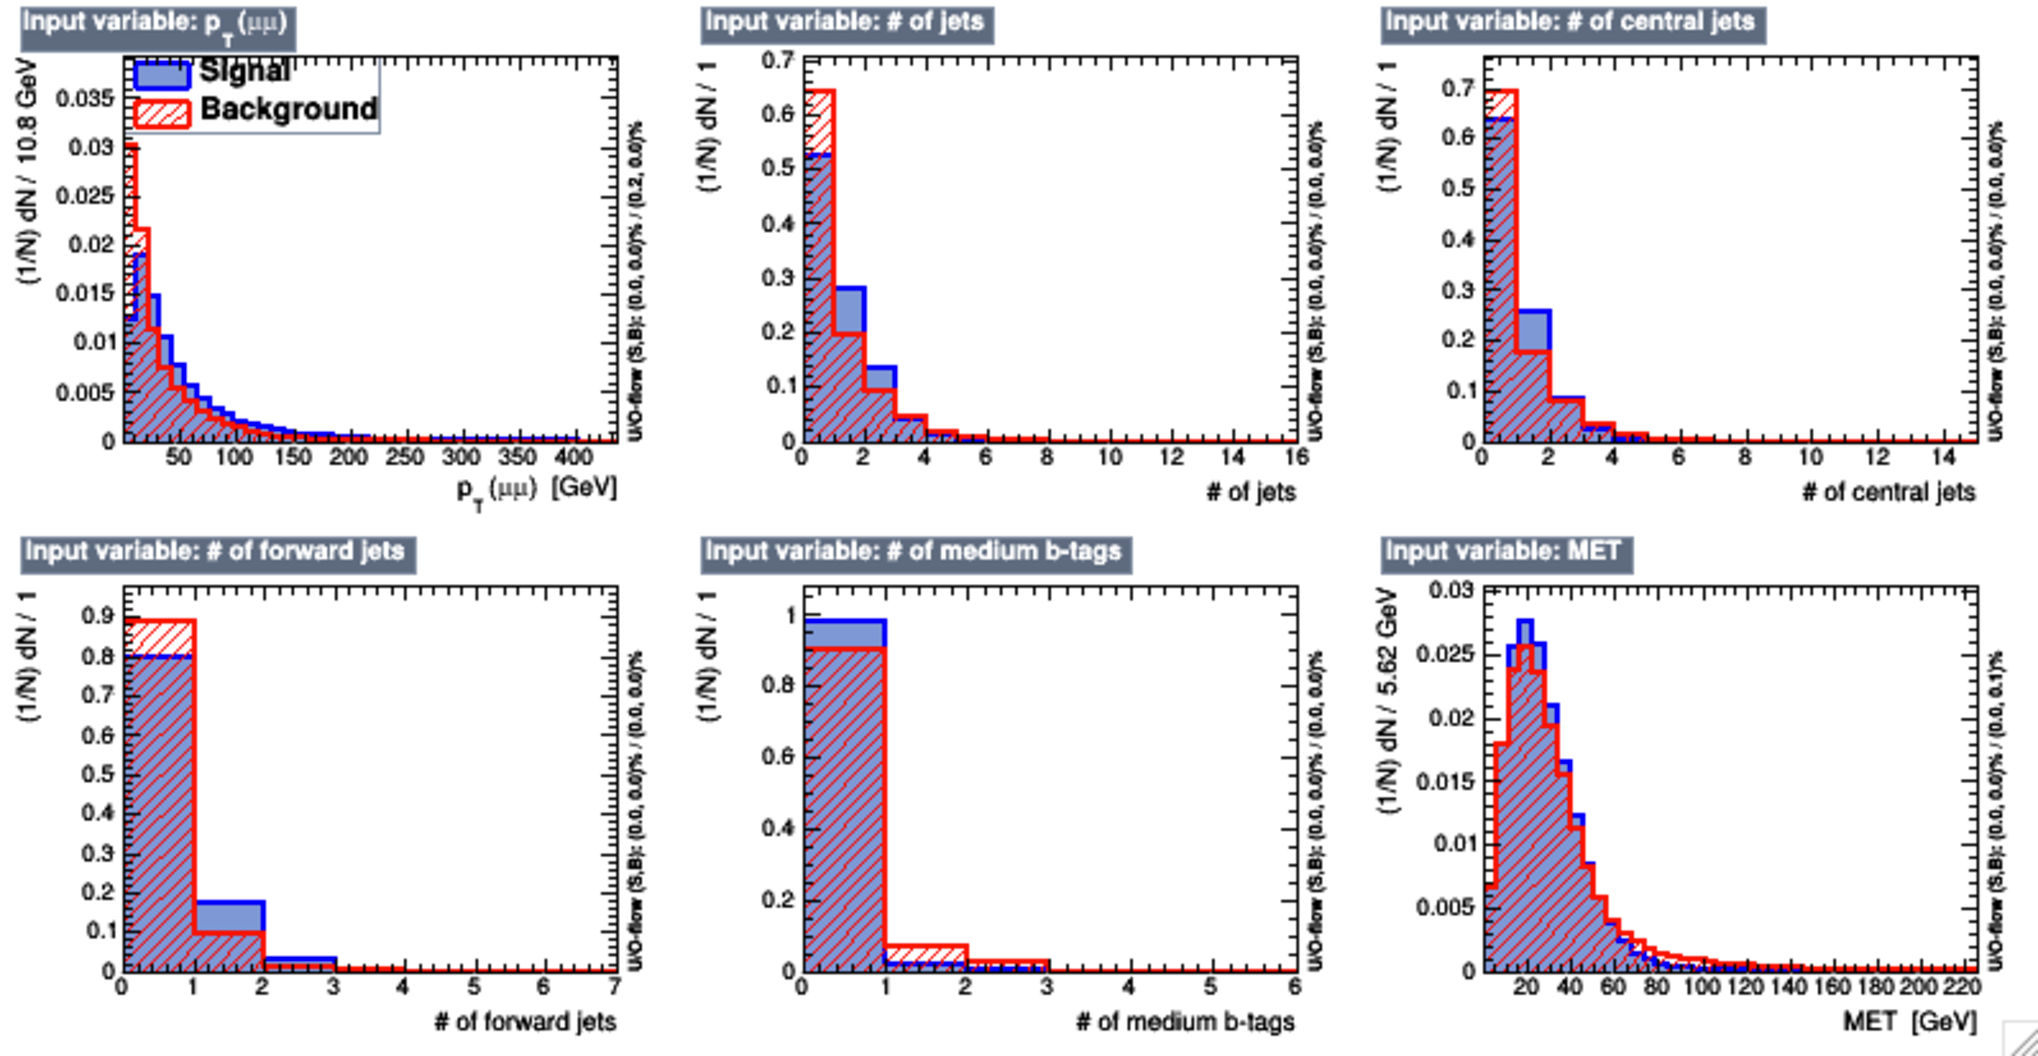
\includegraphics[width=1.0\linewidth]{figures/bdt_training/BDT_in_ge0j_all.pdf}
  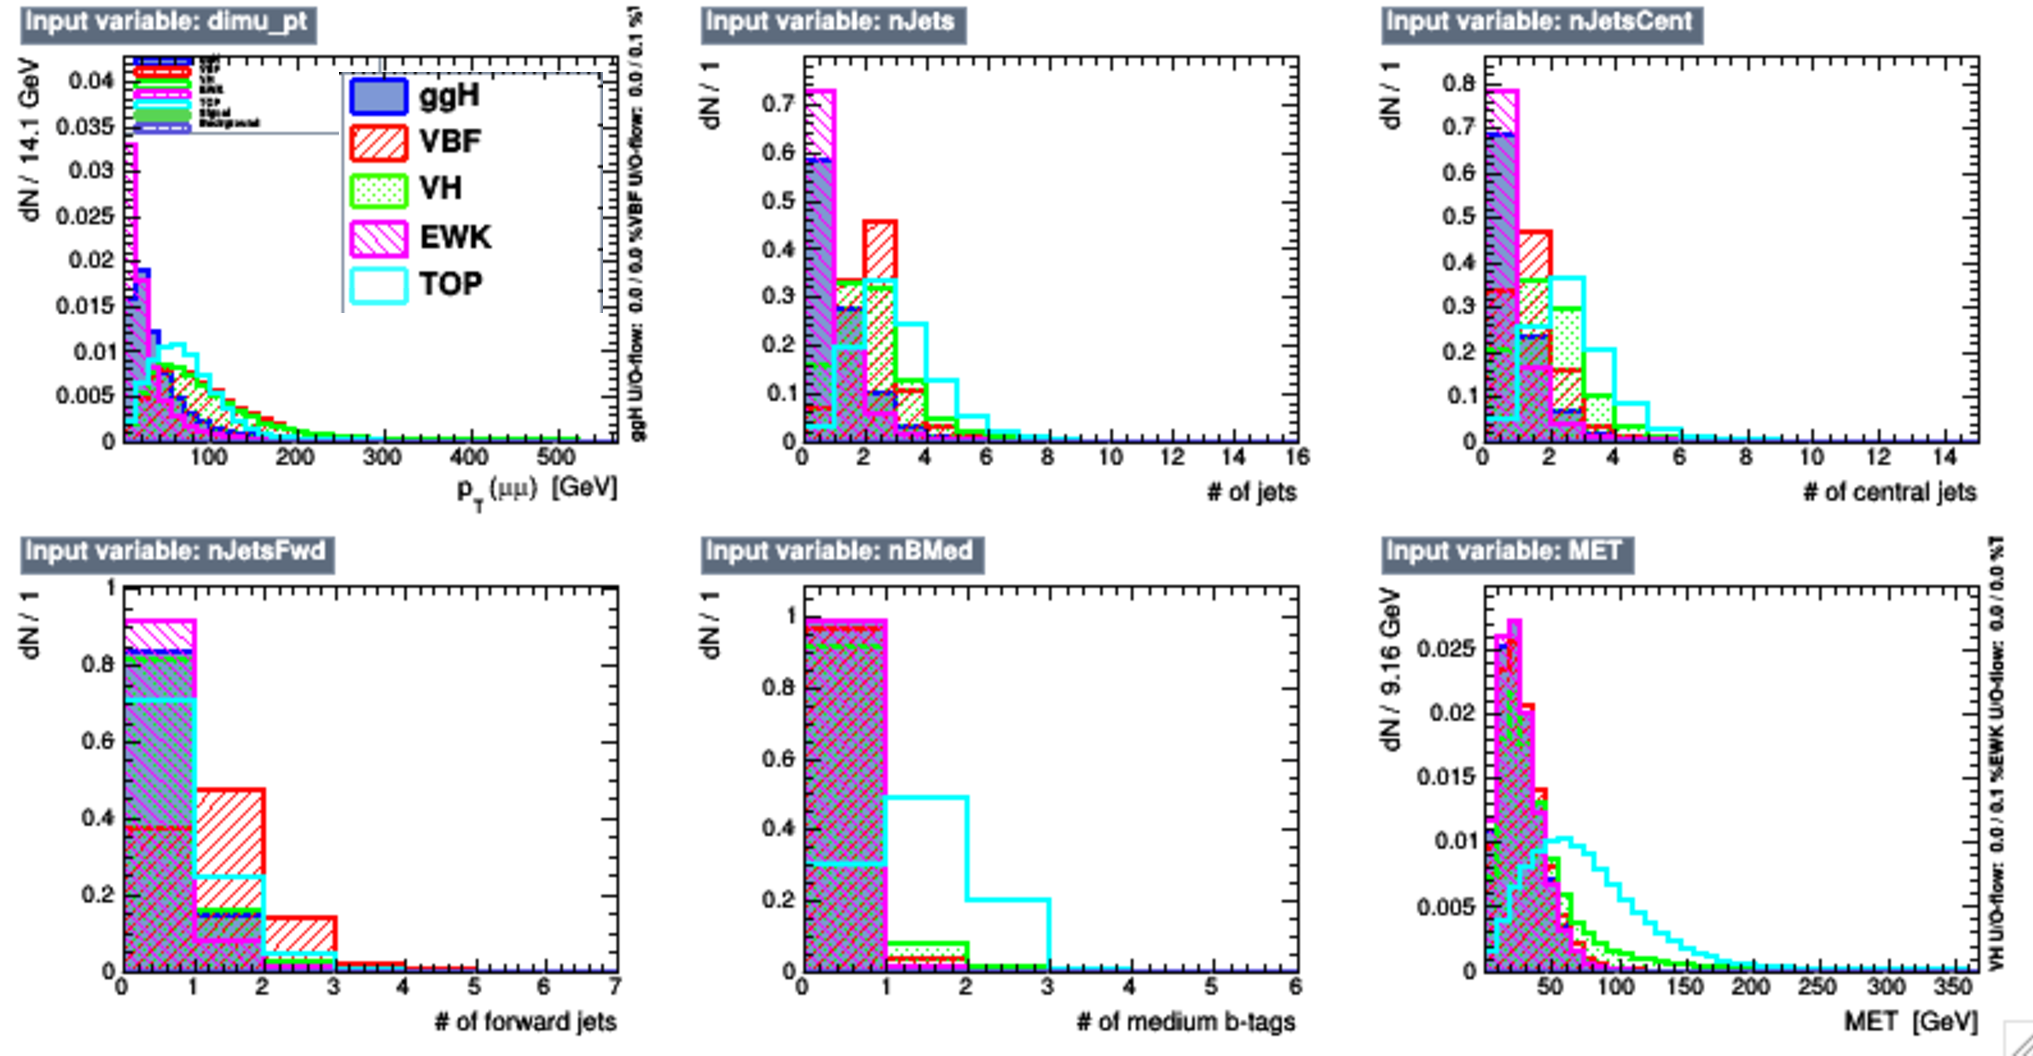
\includegraphics[width=1.0\linewidth]{figures/bdt_training/BDT_in_ge0j_sep.pdf}
  \caption{Some BDT input variables for events with $\ge 0$ jets.
           In the top plots, signal is in blue and background in red.
           In the bottom plots, the gluon-fusion signal is dark blue, VBF is red, and VH is green,
           while Drell--Yan and diboson backgrounds are pink, and \ttbar and single top are light blue.}
  \label{fig:BDT_in_ge0j}
\end{figure}

\begin{figure}
  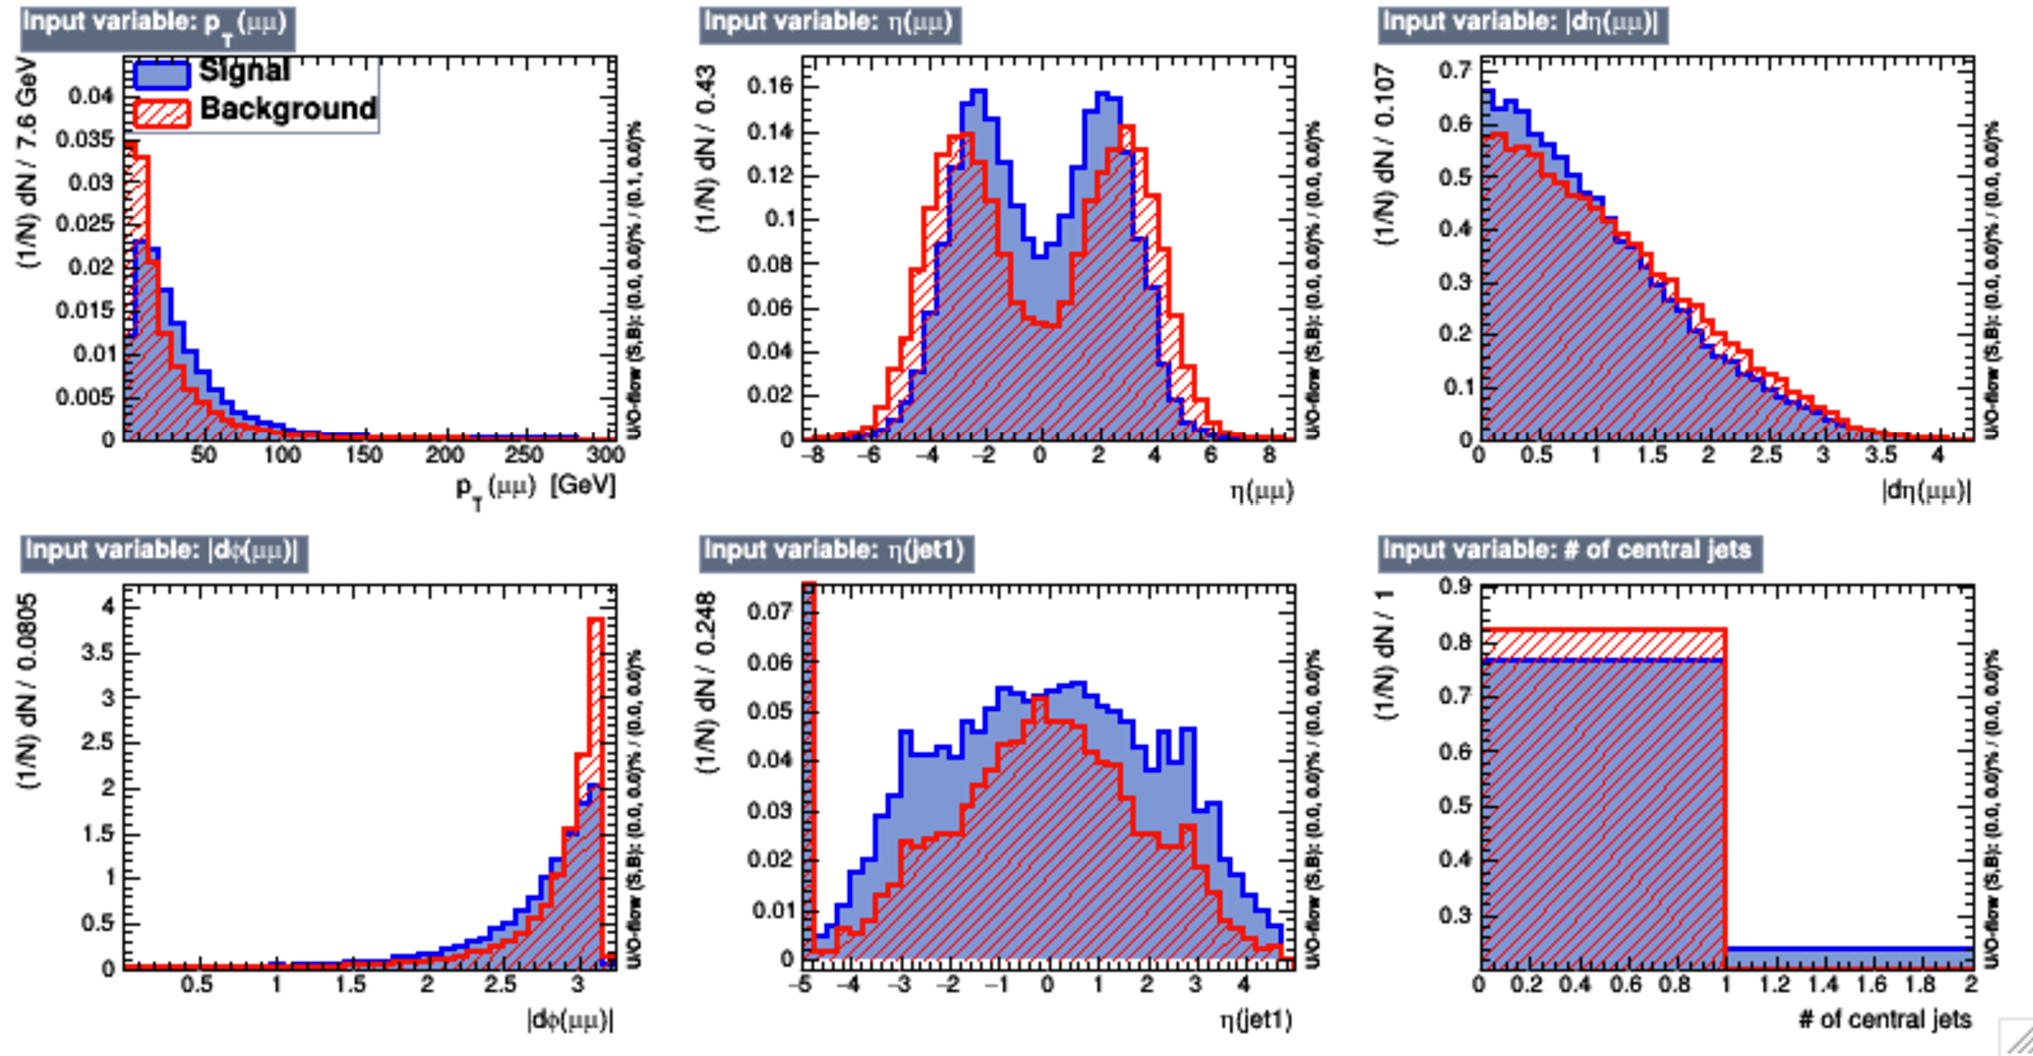
\includegraphics[width=1.0\linewidth]{figures/bdt_training/BDT_in_le1j_all_A.pdf}
  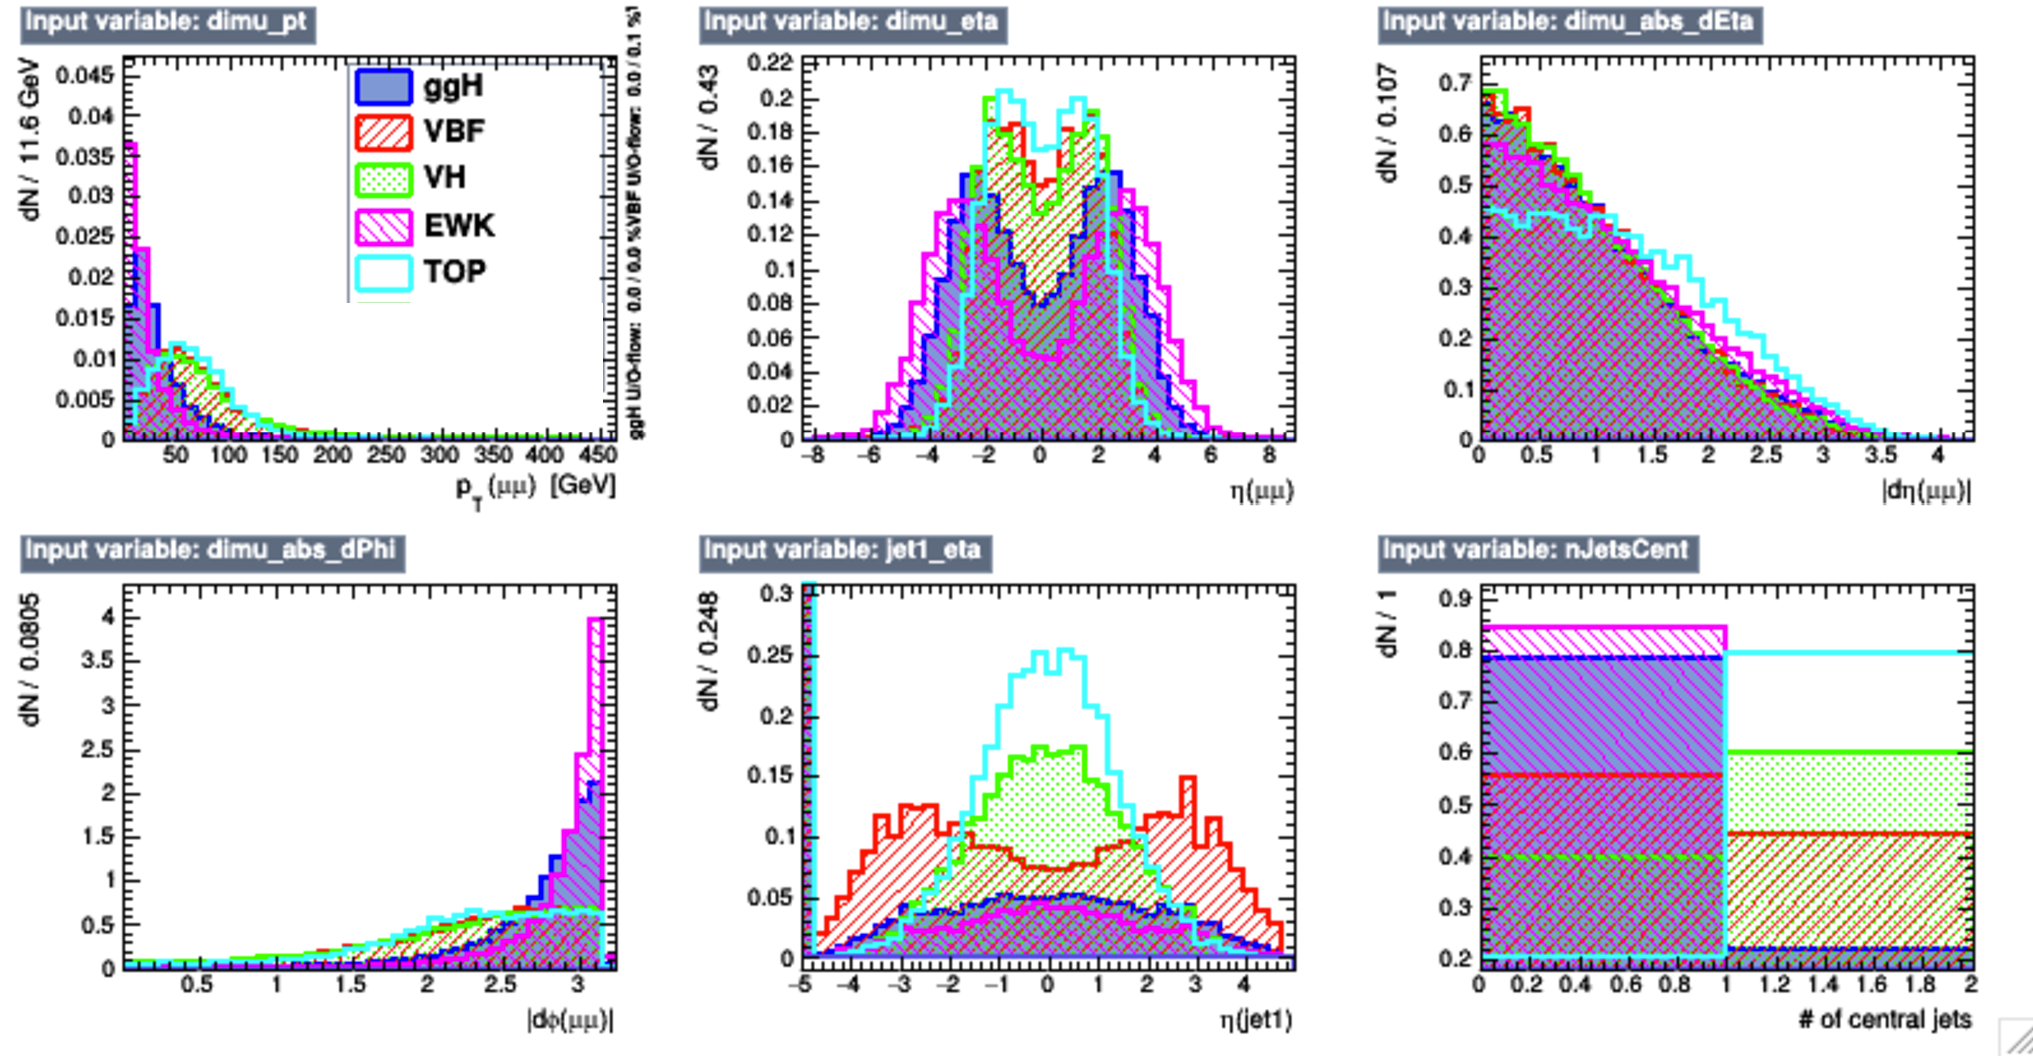
\includegraphics[width=1.0\linewidth]{figures/bdt_training/BDT_in_le1j_sep_A.pdf}
  \caption{Some BDT input variables for events with $\le 1$ jets.
           In the top plots, signal is in blue and background in red.
           In the bottom plots, the gluon-fusion signal is dark blue, VBF is red, and VH is green,
           while Drell--Yan and diboson backgrounds are pink, and \ttbar and single top are light blue.}
  \label{fig:BDT_in_le1j_A}
\end{figure}

\begin{figure}
  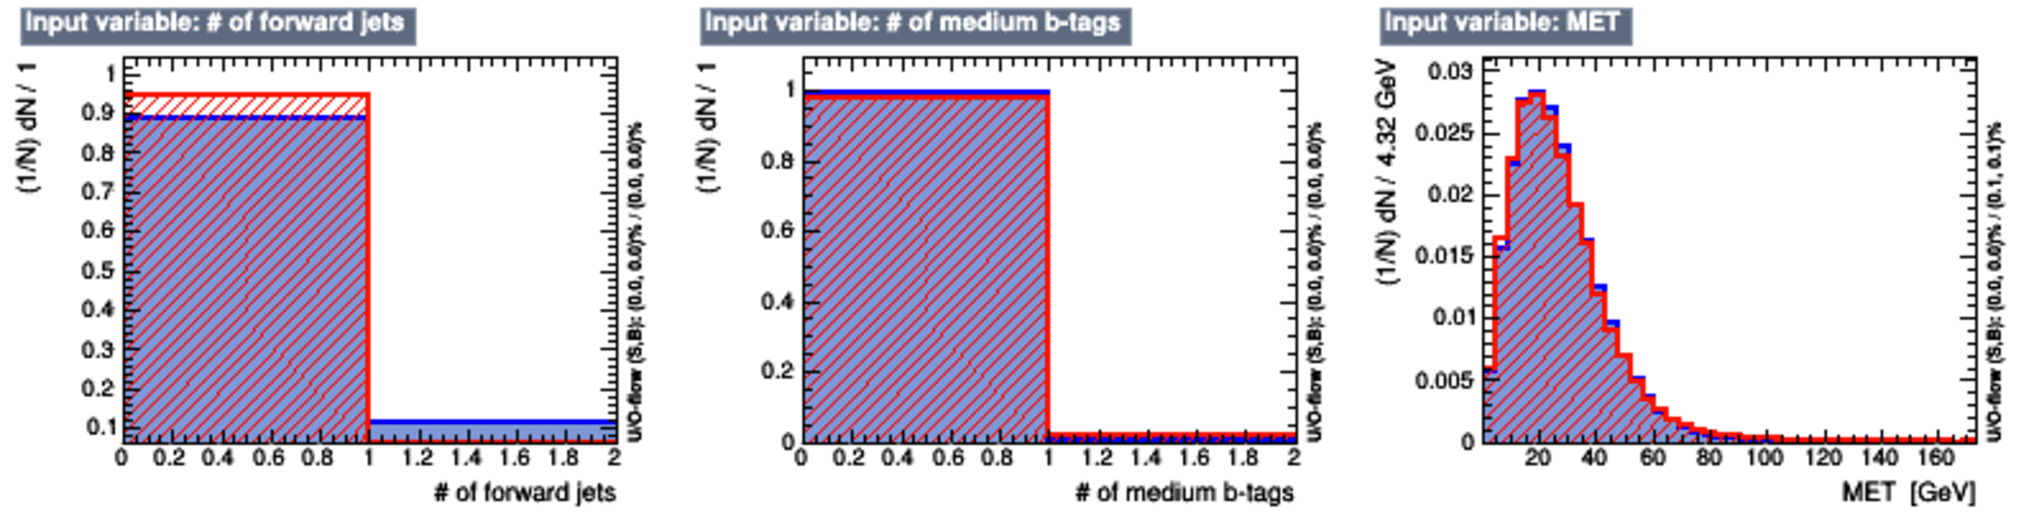
\includegraphics[width=1.0\linewidth]{figures/bdt_training/BDT_in_le1j_all_B.pdf}
  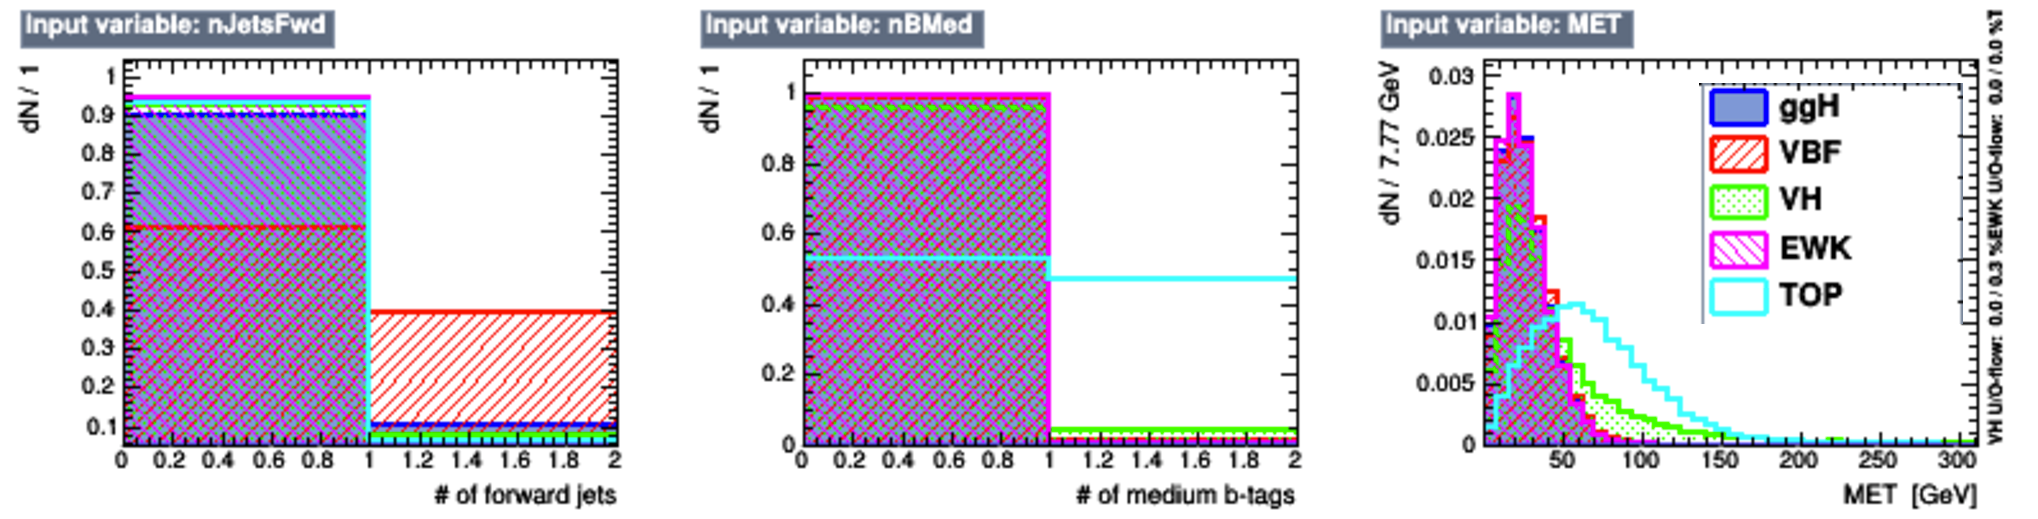
\includegraphics[width=1.0\linewidth]{figures/bdt_training/BDT_in_le1j_sep_B.pdf}
  \caption{Some BDT input variables for events with $\le 1$ jets.
           In the top plots, signal is in blue and background in red.
           In the bottom plots, the gluon-fusion signal is dark blue, VBF is red, and VH is green,
           while Drell--Yan and diboson backgrounds are pink, and \ttbar and single top are light blue.}
  \label{fig:BDT_in_le1j_B}
\end{figure}

\begin{figure}
  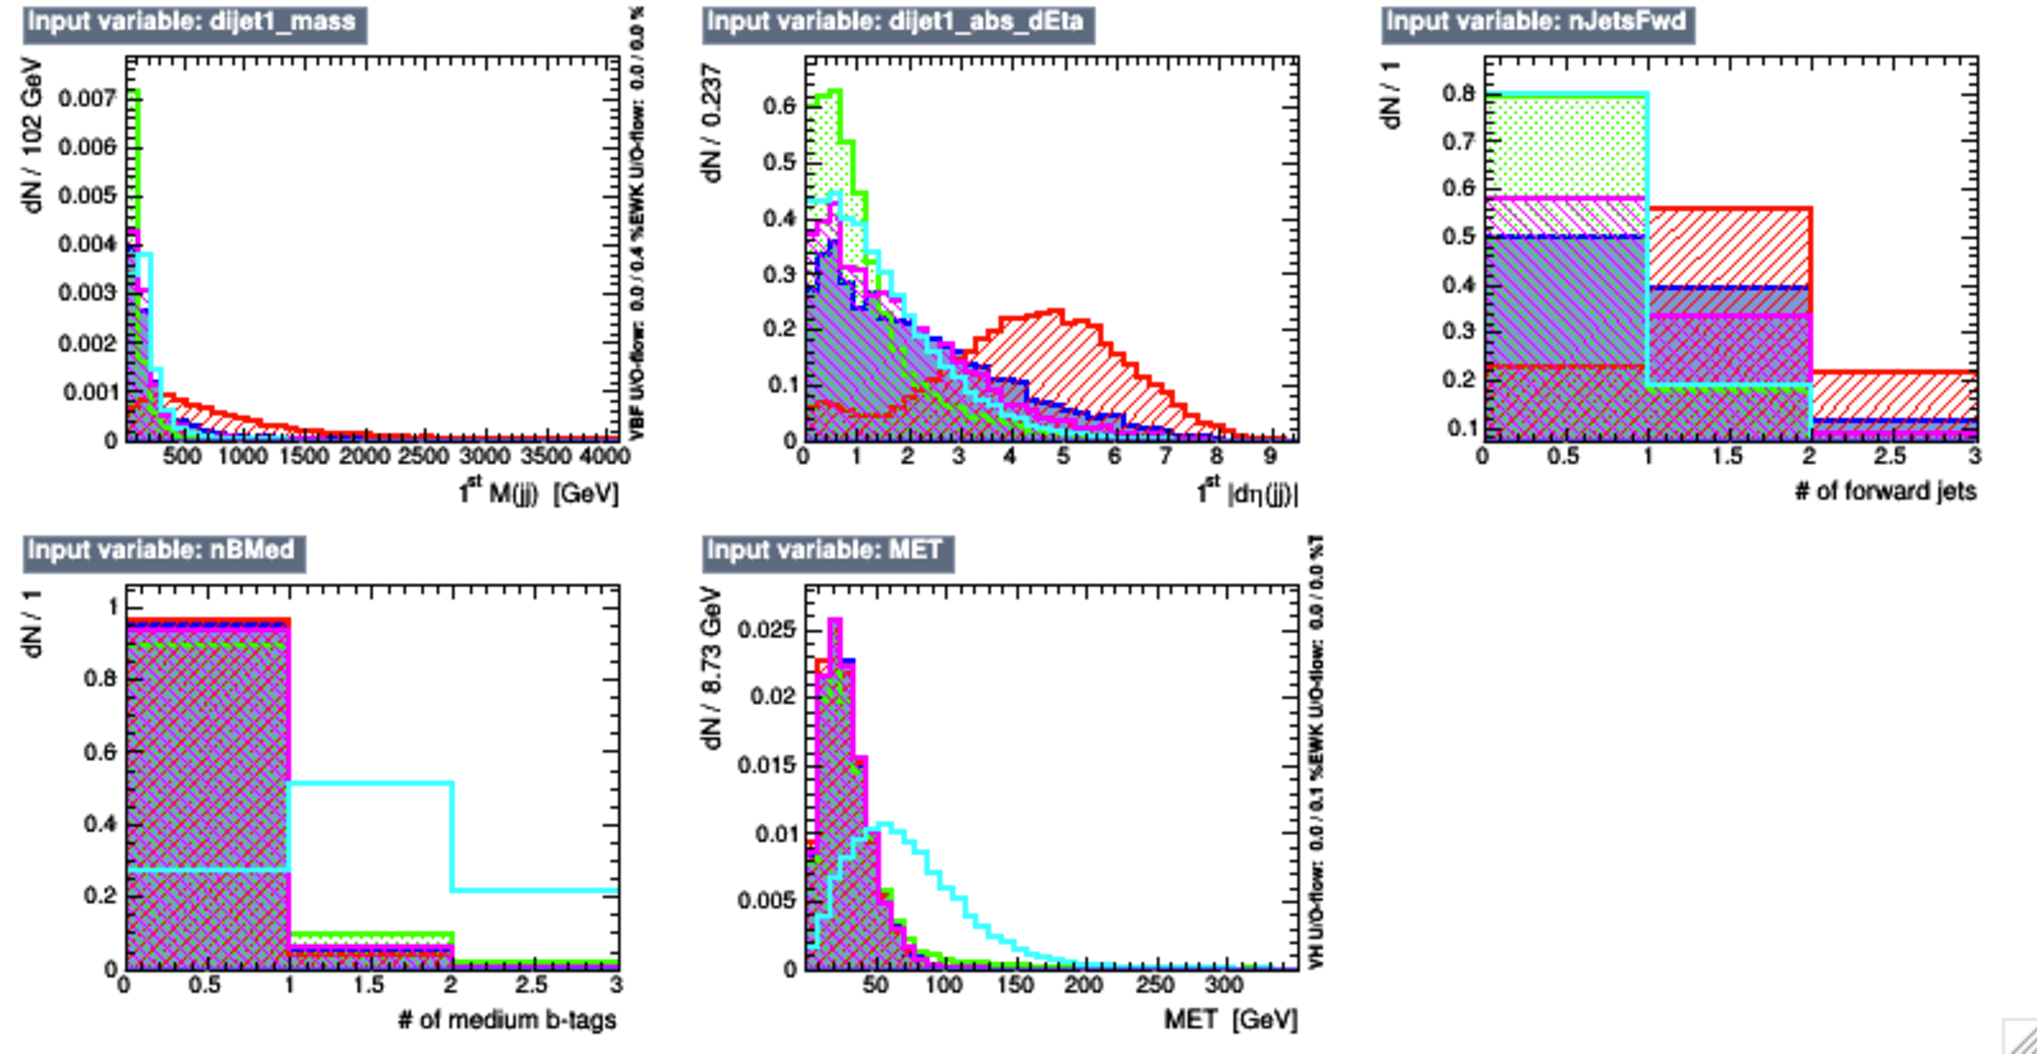
\includegraphics[width=1.0\linewidth]{figures/bdt_training/BDT_in_eq2j_sep_B.pdf}
  \caption{Some BDT input variables for events with $= 2$ jets.
           The gluon-fusion signal is dark blue, VBF is red, and VH is green,
           while Drell--Yan and diboson backgrounds are pink, and \ttbar and single top are light blue.}
  \label{fig:BDT_in_eq2j_B}
\end{figure}

\begin{figure}
  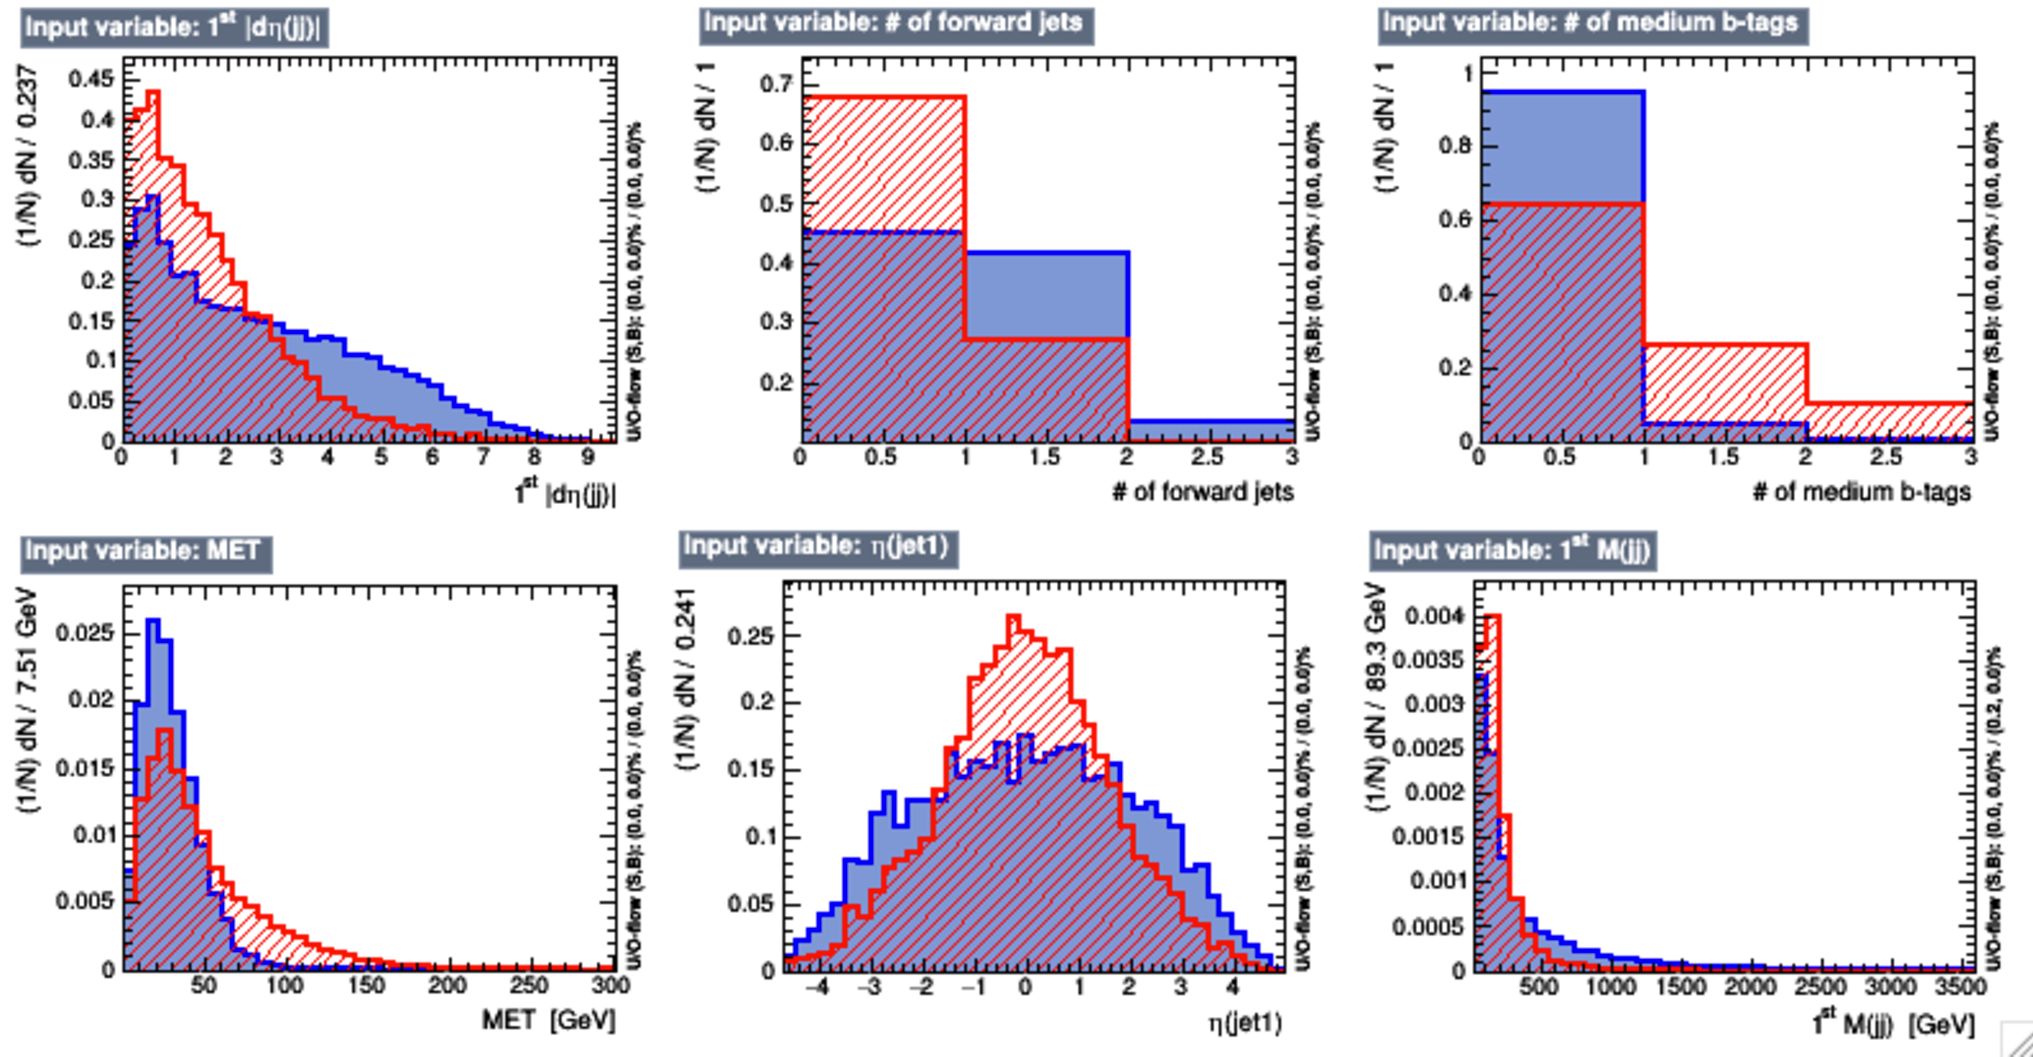
\includegraphics[width=1.0\linewidth]{figures/bdt_training/BDT_in_eq2j_all_A.pdf}
  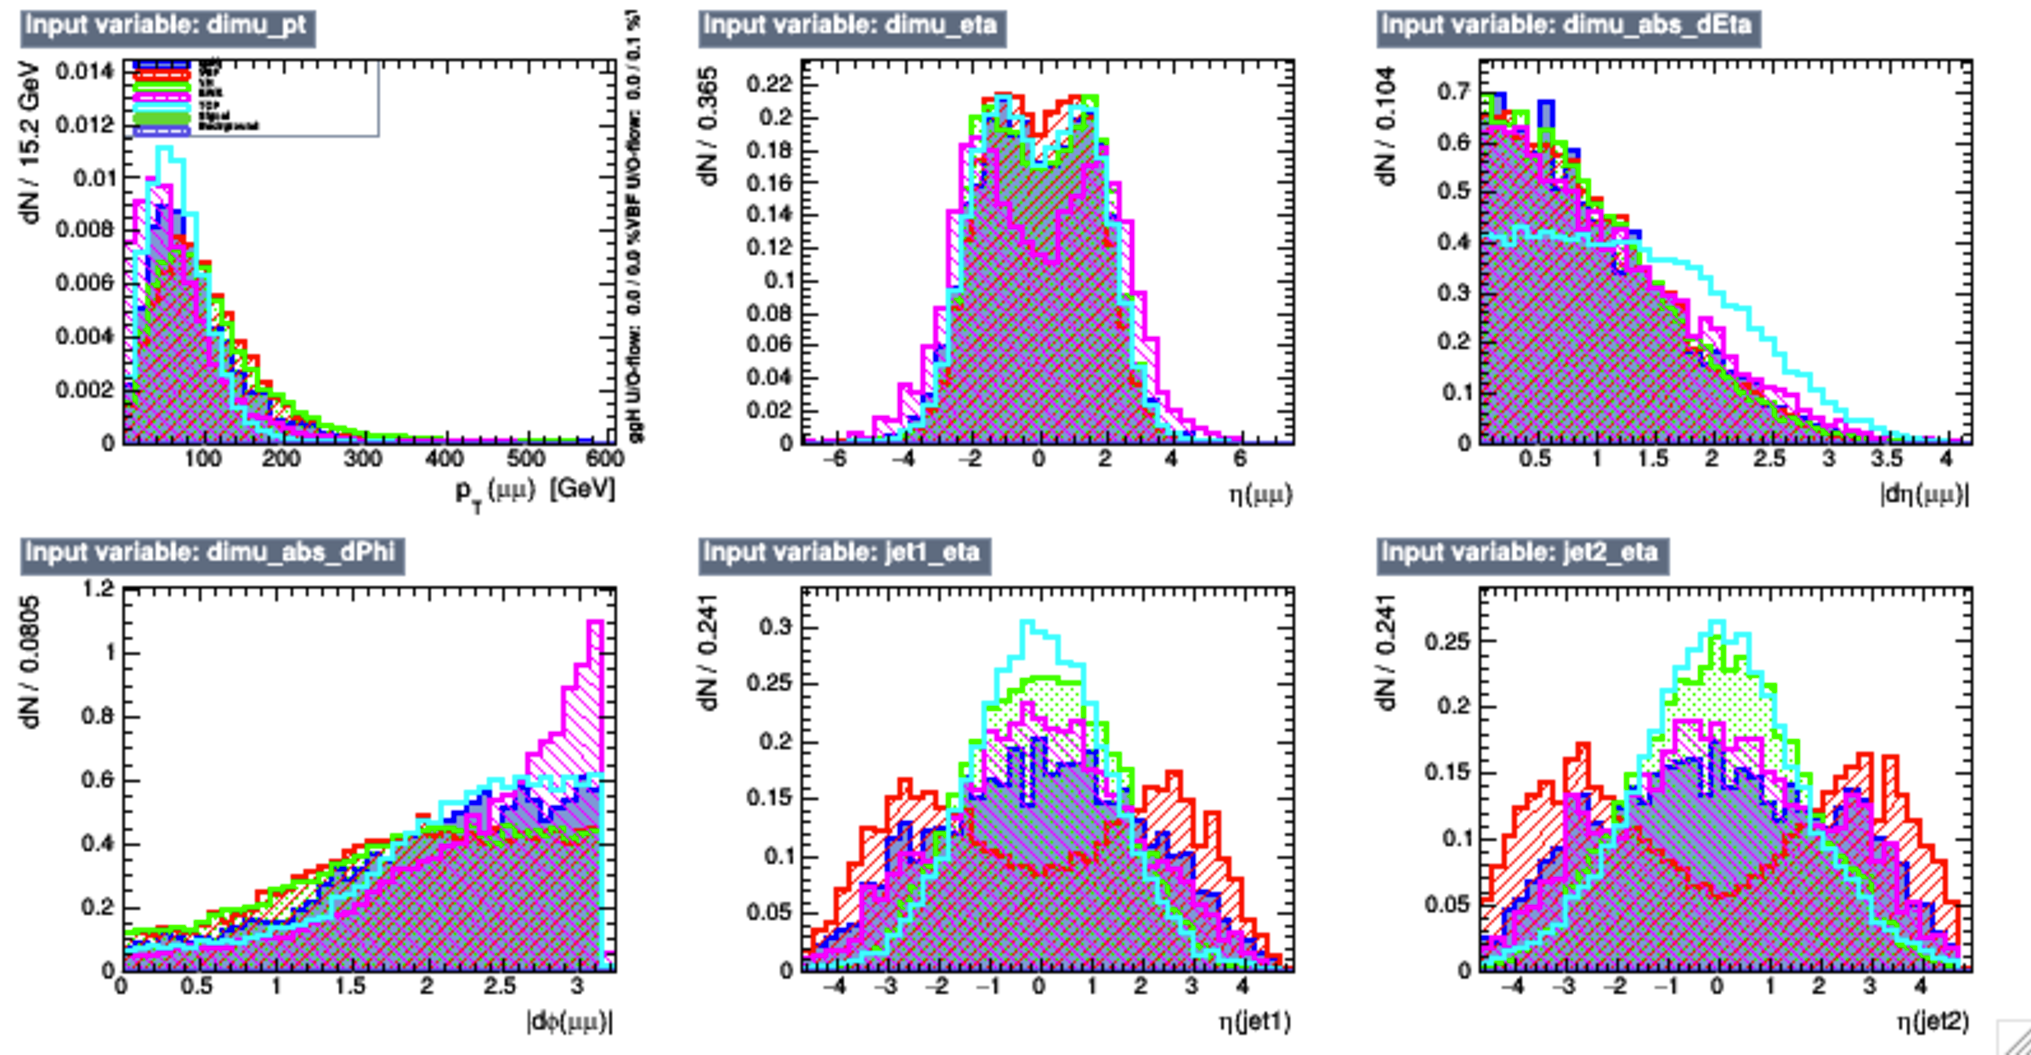
\includegraphics[width=1.0\linewidth]{figures/bdt_training/BDT_in_eq2j_sep_A.pdf}
  \caption{Some BDT input variables for events with $= 2$ jets.
           In the top plots, signal is in blue and background in red.
           In the bottom plots, the gluon-fusion signal is dark blue, VBF is red, and VH is green,
           while Drell--Yan and diboson backgrounds are pink, and \ttbar and single top are light blue.}
  \label{fig:BDT_in_eq2j_A}
\end{figure}

\begin{figure}
  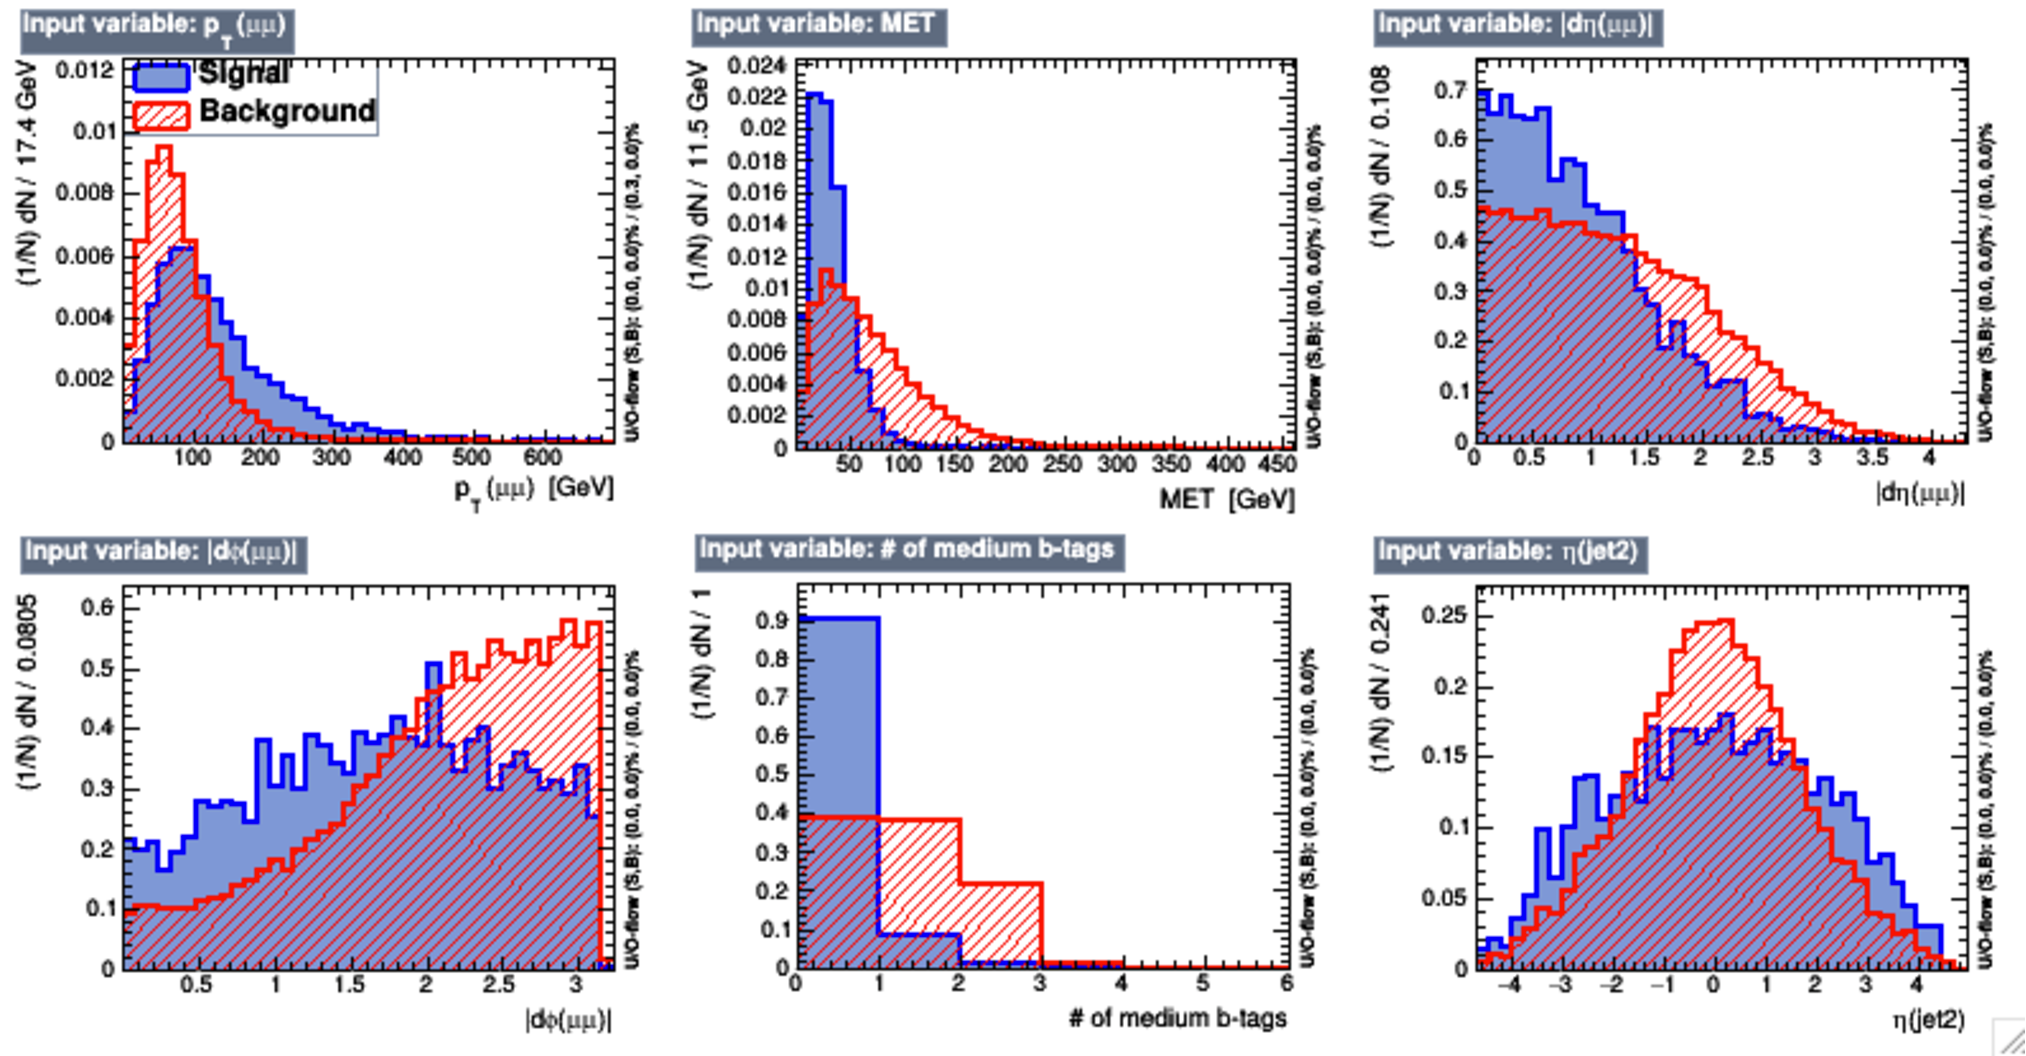
\includegraphics[width=1.0\linewidth]{figures/bdt_training/BDT_in_ge3j_all_A.pdf}
  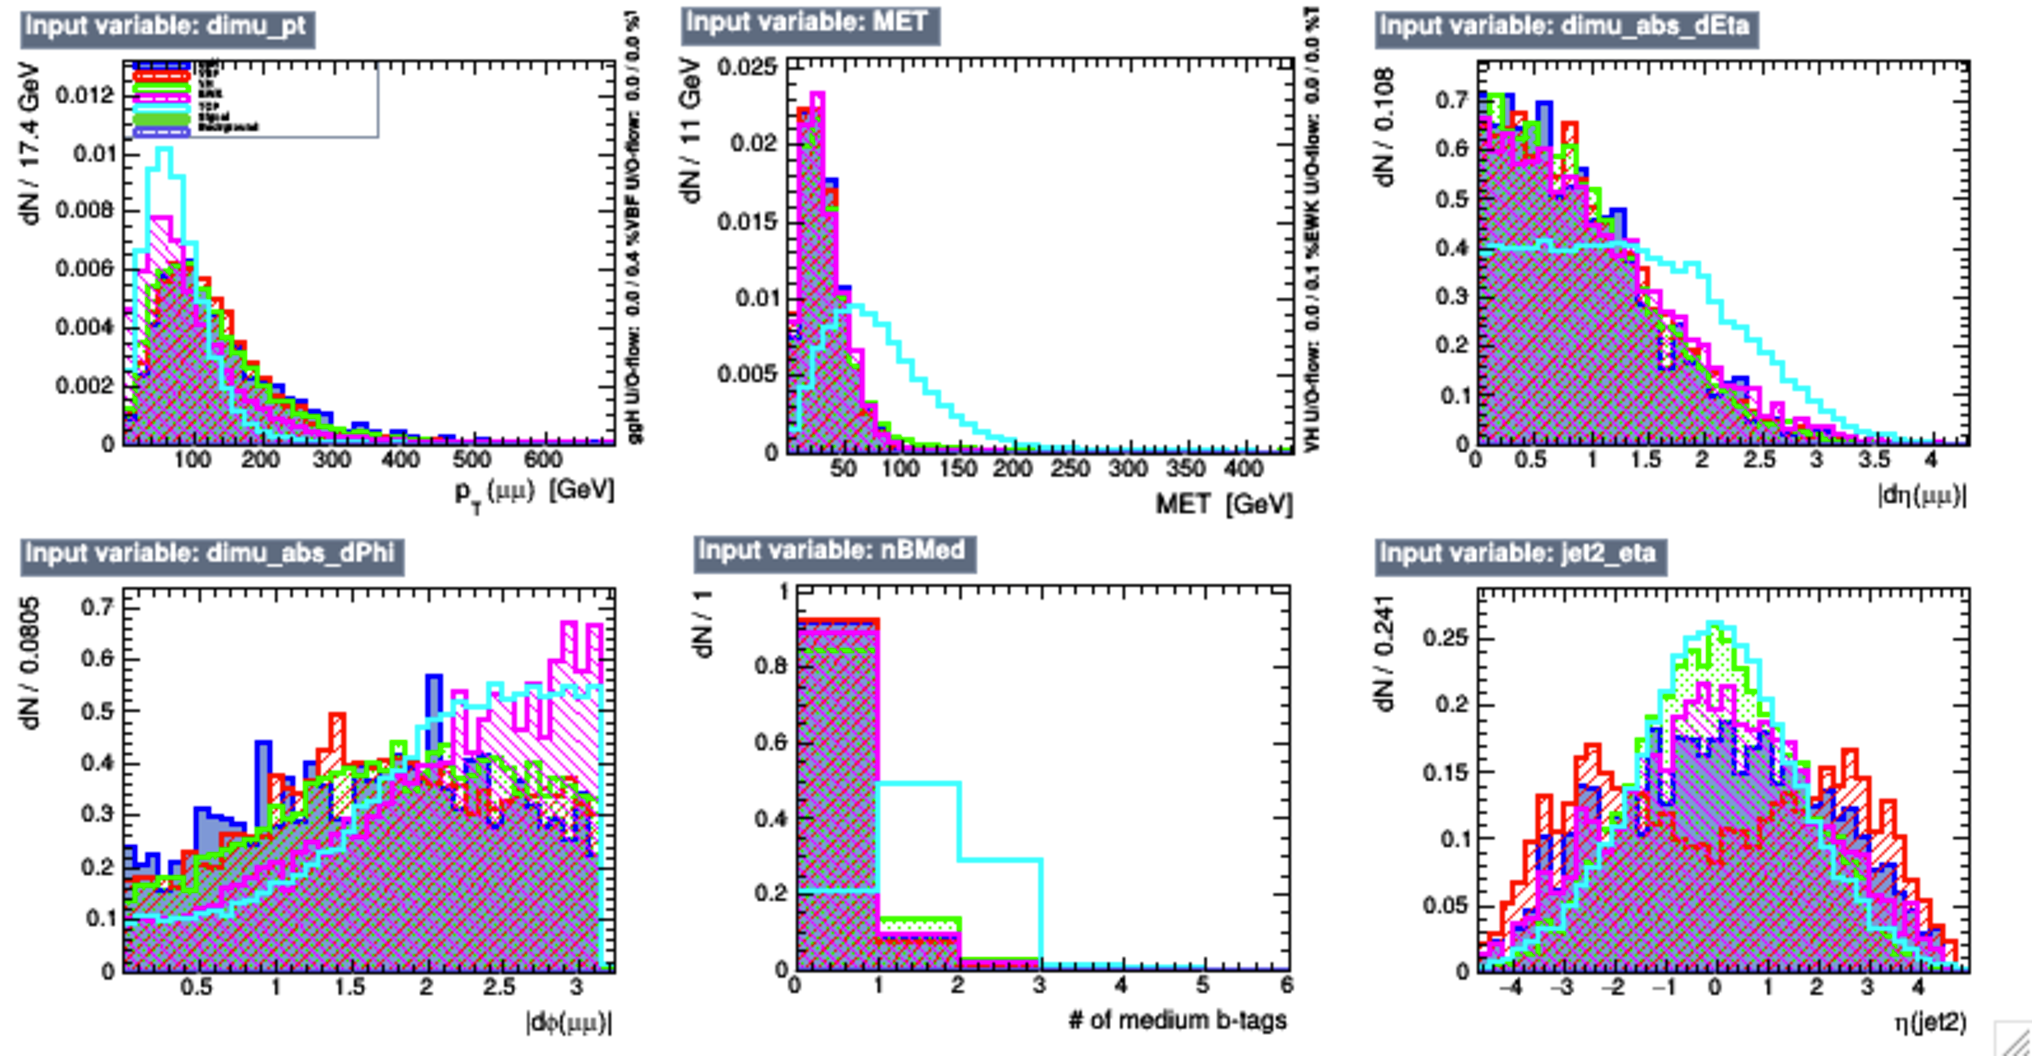
\includegraphics[width=1.0\linewidth]{figures/bdt_training/BDT_in_ge3j_sep_A.pdf}
  \caption{Some BDT input variables for events with $\ge 3$ jets.
           In the top plots, signal is in blue and background in red.
           In the bottom plots, the gluon-fusion signal is dark blue, VBF is red, and VH is green,
           while Drell--Yan and diboson backgrounds are pink, and \ttbar and single top are light blue.}
  \label{fig:BDT_in_ge3j_A}
\end{figure}

\begin{figure}
  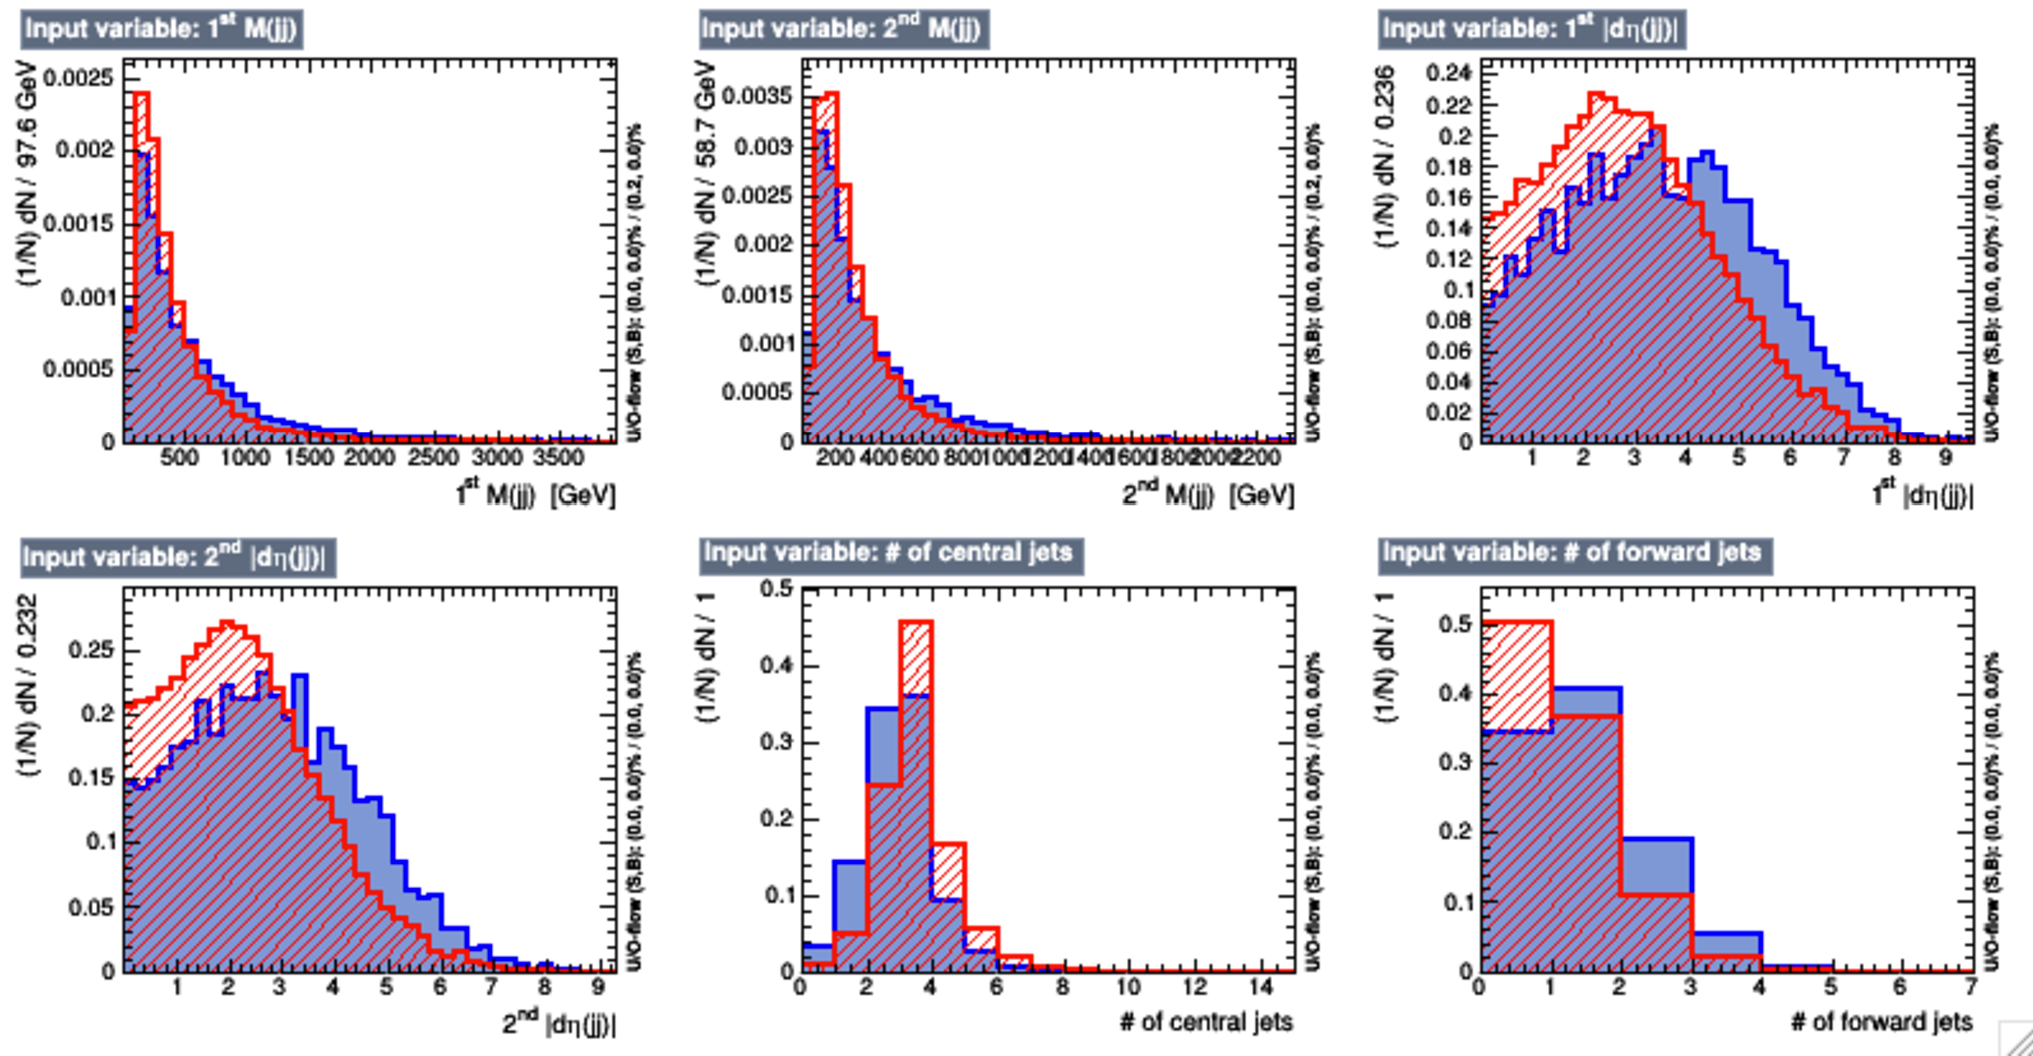
\includegraphics[width=1.0\linewidth]{figures/bdt_training/BDT_in_ge3j_all_B.pdf}
  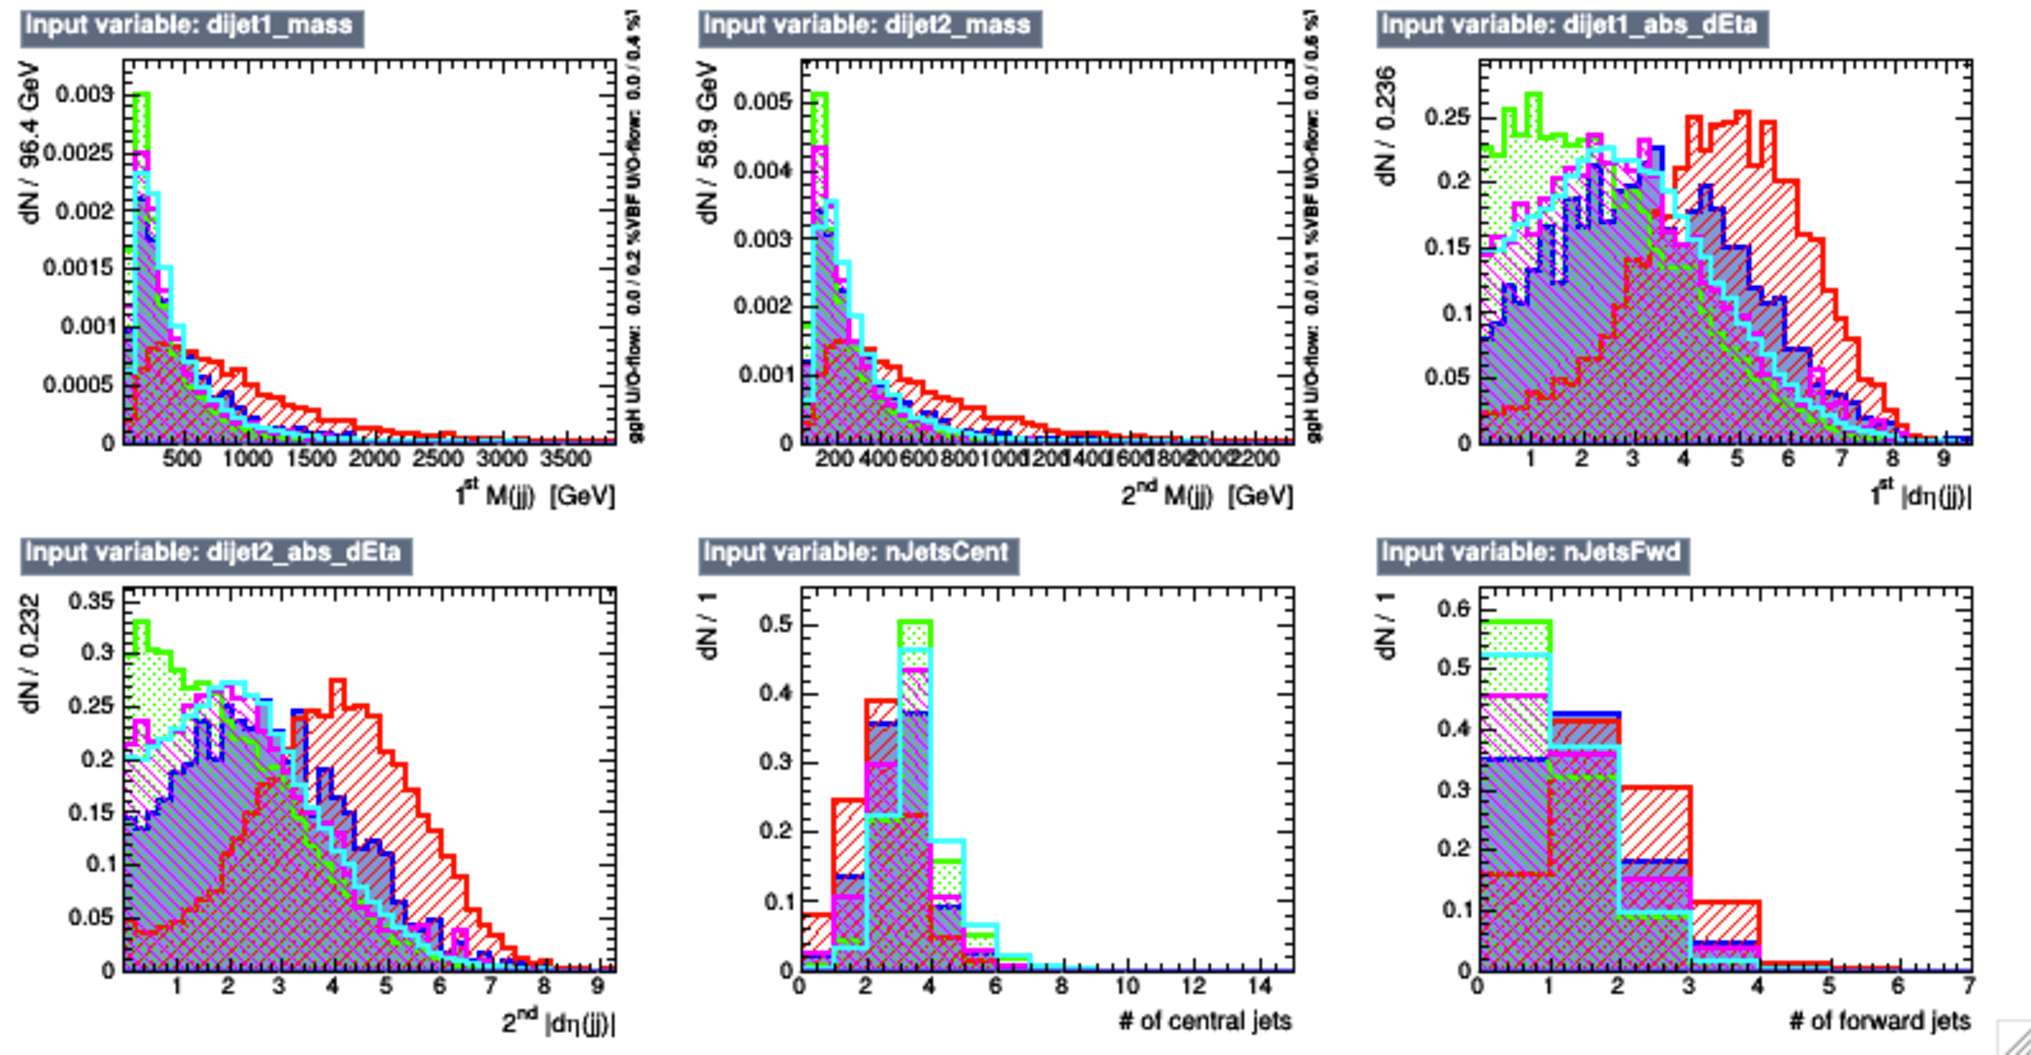
\includegraphics[width=1.0\linewidth]{figures/bdt_training/BDT_in_ge3j_sep_B.pdf}
  \caption{Some BDT input variables for events with $\ge 3$ jets.
           In the top plots, signal is in blue and background in red.
           In the bottom plots, the gluon-fusion signal is dark blue, VBF is red, and VH is green,
           while Drell--Yan and diboson backgrounds are pink, and \ttbar and single top are light blue.}
  \label{fig:BDT_in_ge3j_B}
\end{figure}

\clearpage

The BDT output distributions for both the inclusive and $\le 1$, $= 2$, and $\ge 3$
jet trainings can be seen in Figure~\ref{fig:BDT_out}, with the corresponding ROC curves
in Figure~\ref{fig:BDT_ROC}.  We also performed a multi-classification which assigned
separate BDT scores for each of the signal and background classes: ggH, VBF, VH, EWK,
and TOP.  In the end, the binary signal--background classification algorithm, trained
on the inclusve $\ge 0$ jets sample of events, provided a signal--background separation
which was as good as any scheme using either the separate-jet trainings or the
multi-classification algorithm.

\begin{figure}
  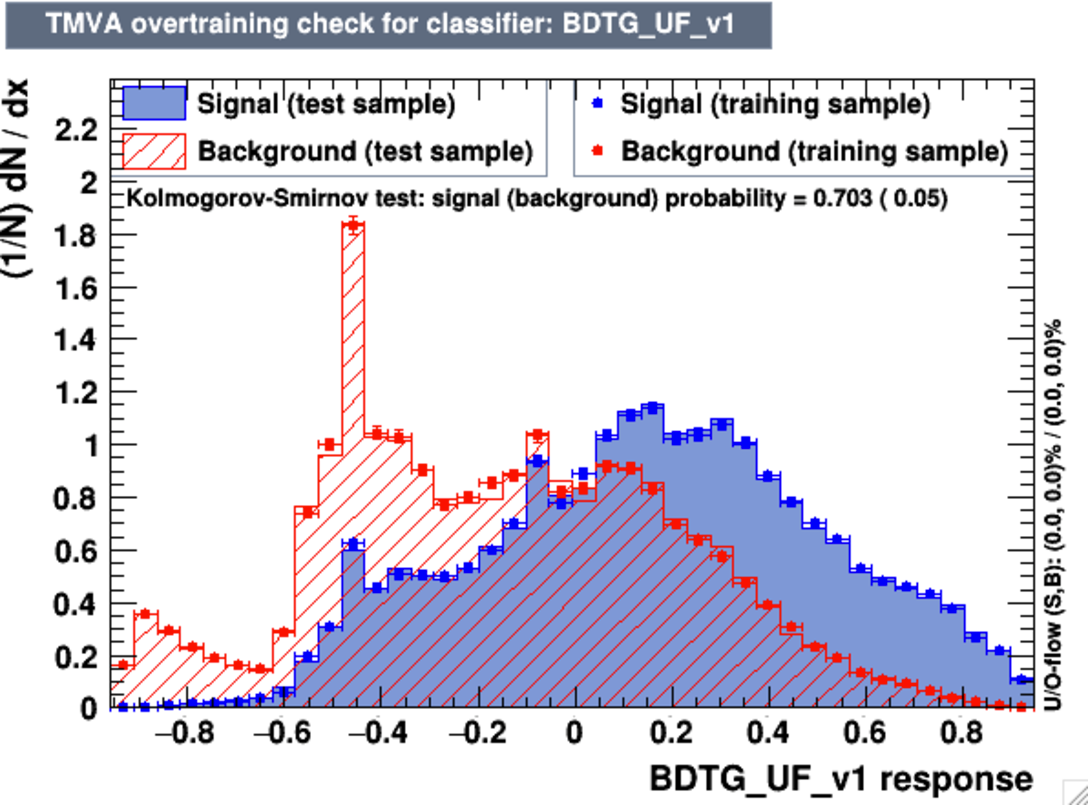
\includegraphics[width=0.5\linewidth]{figures/bdt_training/BDT_out_ge0j_all.pdf}
  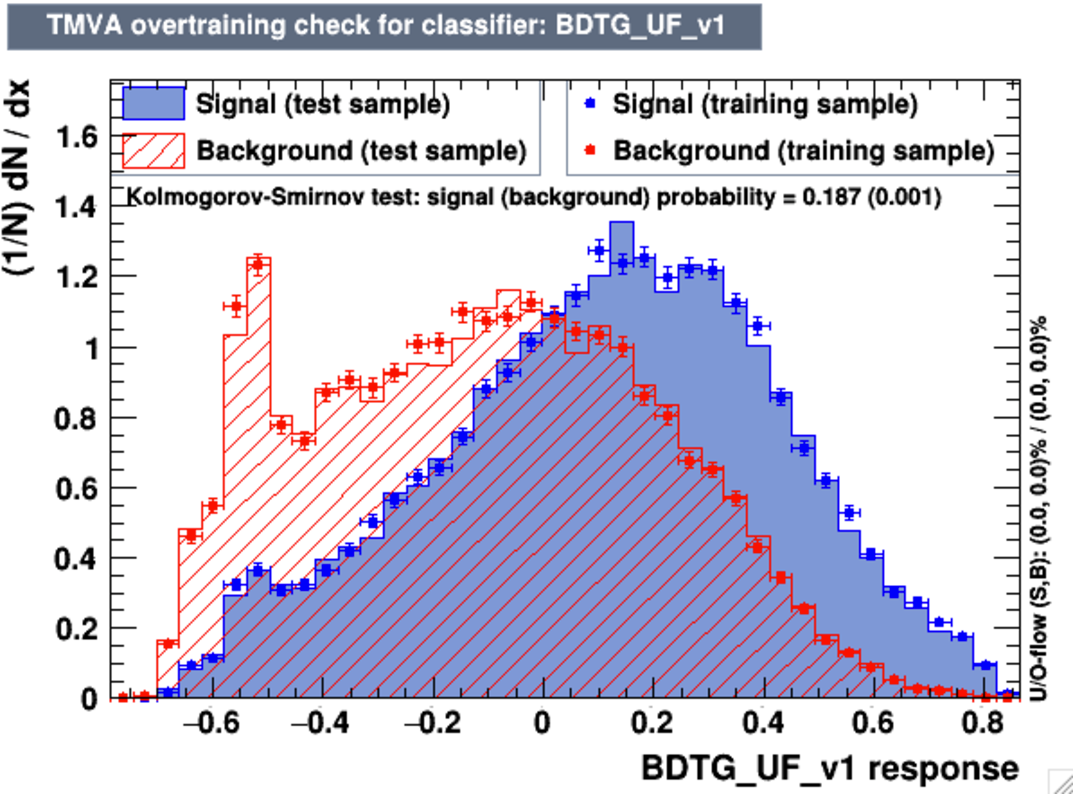
\includegraphics[width=0.5\linewidth]{figures/bdt_training/BDT_out_le1j_all.pdf}
  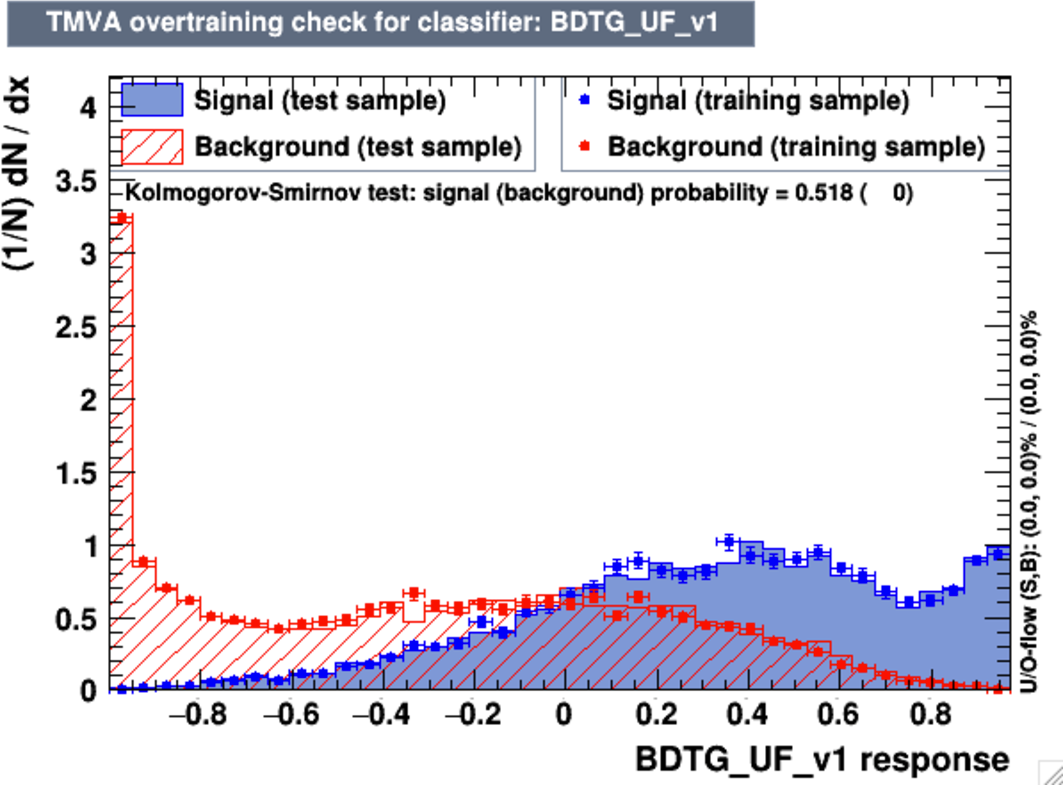
\includegraphics[width=0.5\linewidth]{figures/bdt_training/BDT_out_eq2j_all.pdf}
  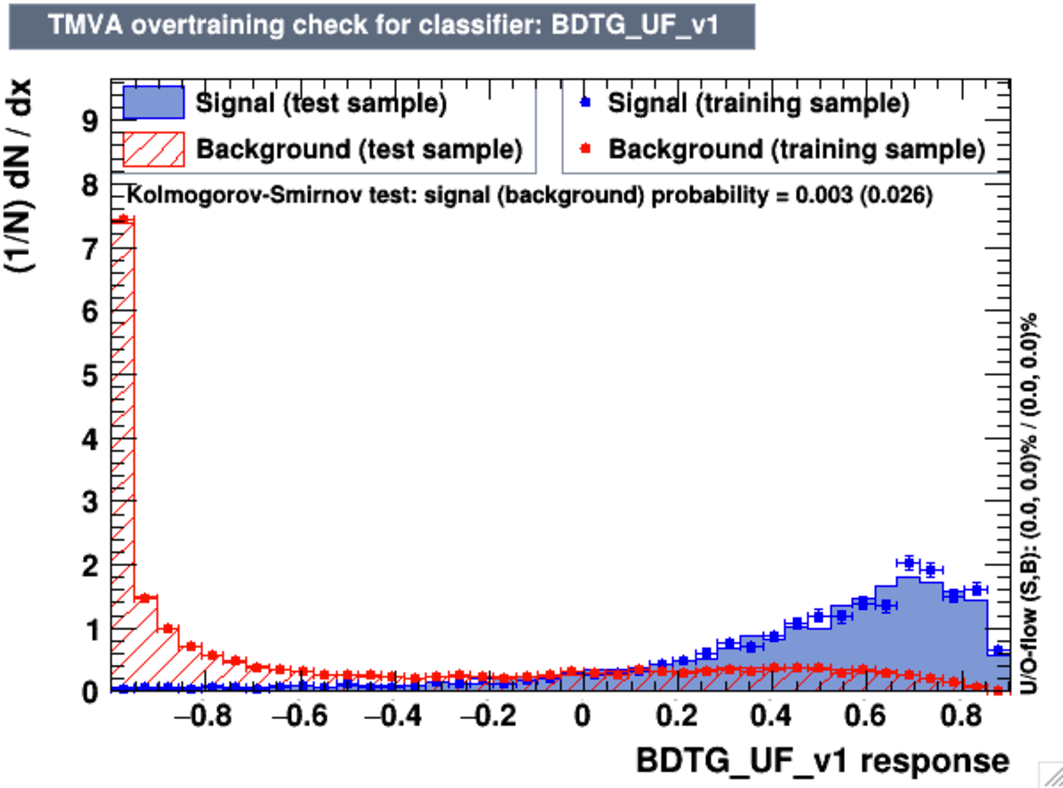
\includegraphics[width=0.5\linewidth]{figures/bdt_training/BDT_out_ge3j_all.pdf}
  \caption{The BDT output score for events with $\ge 0$ jets (top left), $\leq 1$ jet (top right),
           $= 2$ jets (bottom left), and $\ge 3$ jets (bottom right).}
  \label{fig:BDT_out}
\end{figure}

\begin{figure}
  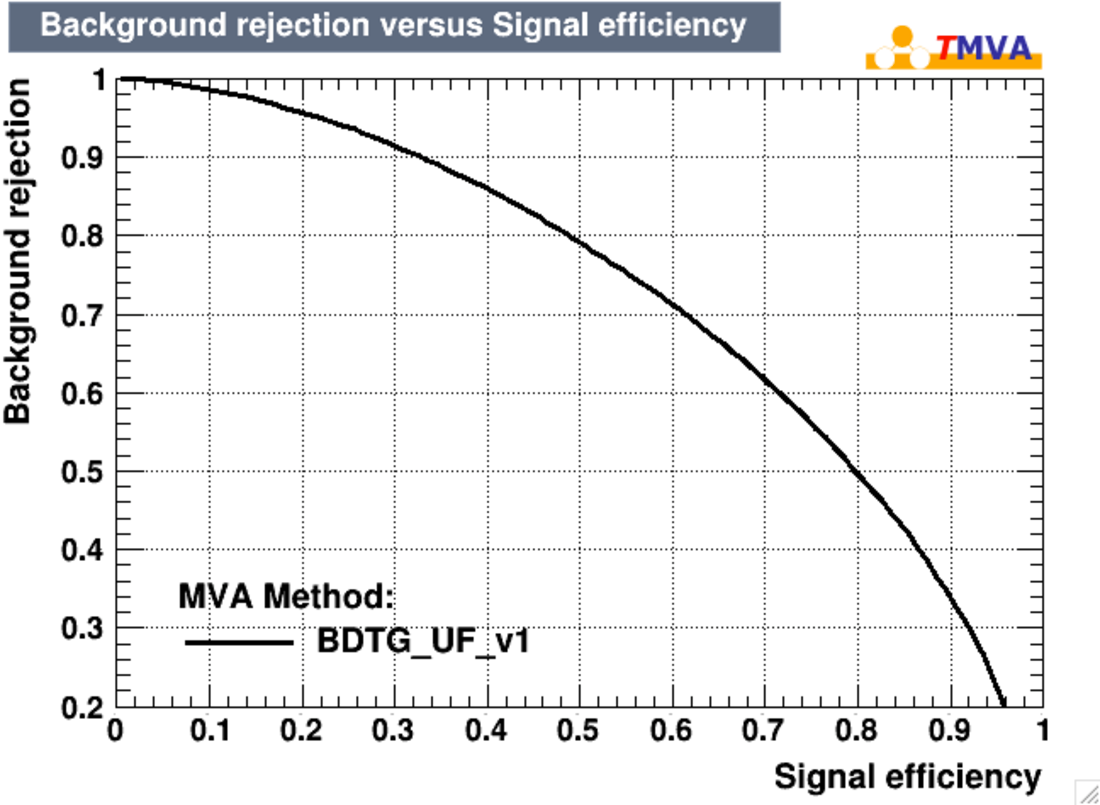
\includegraphics[width=0.5\linewidth]{figures/bdt_training/BDT_ROC_ge0j_all.pdf}
  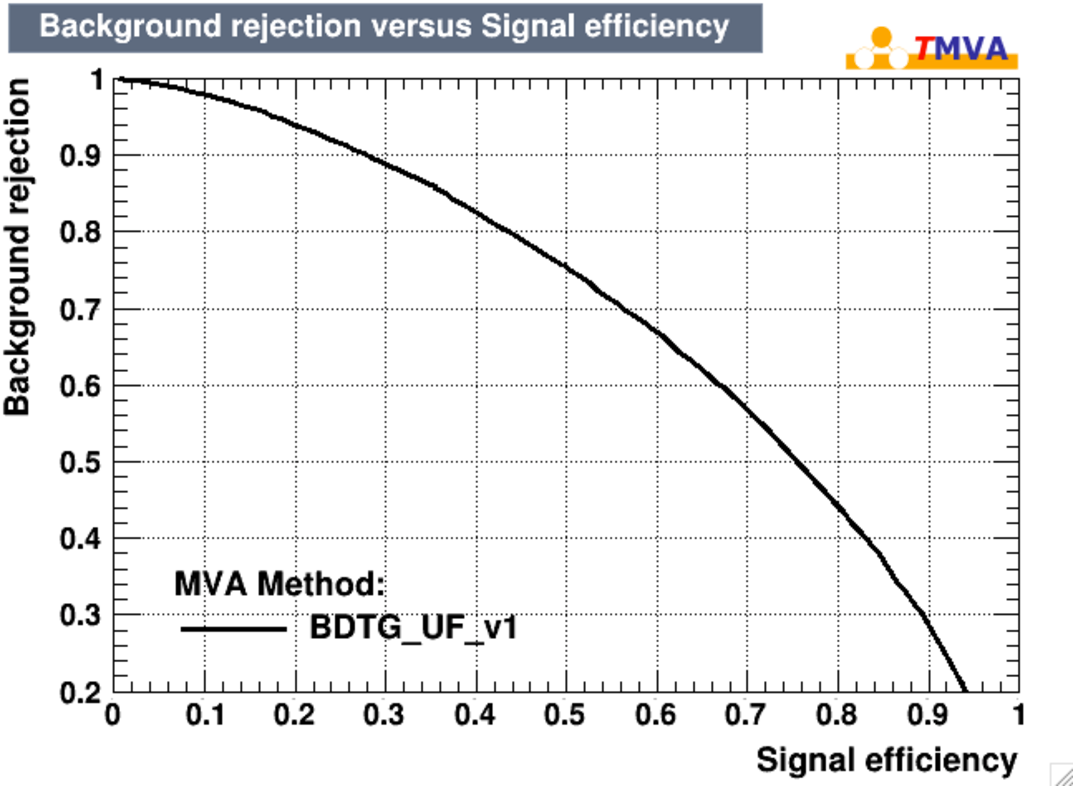
\includegraphics[width=0.5\linewidth]{figures/bdt_training/BDT_ROC_le1j_all.pdf}
  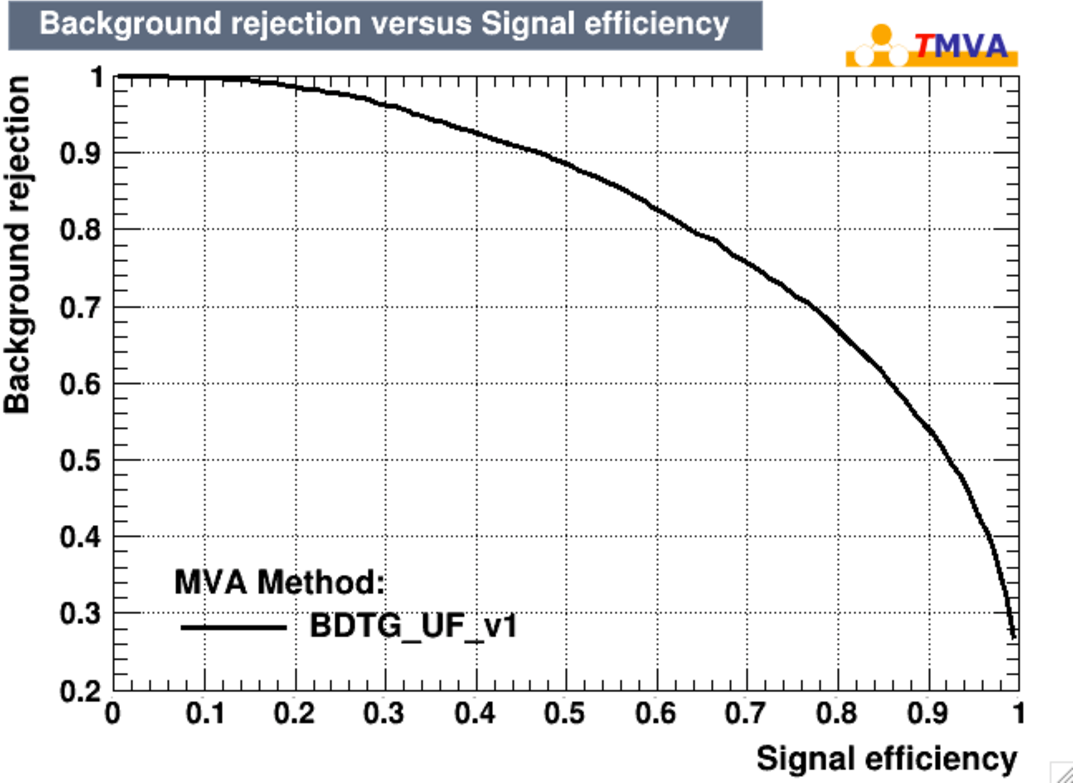
\includegraphics[width=0.5\linewidth]{figures/bdt_training/BDT_ROC_eq2j_all.pdf}
  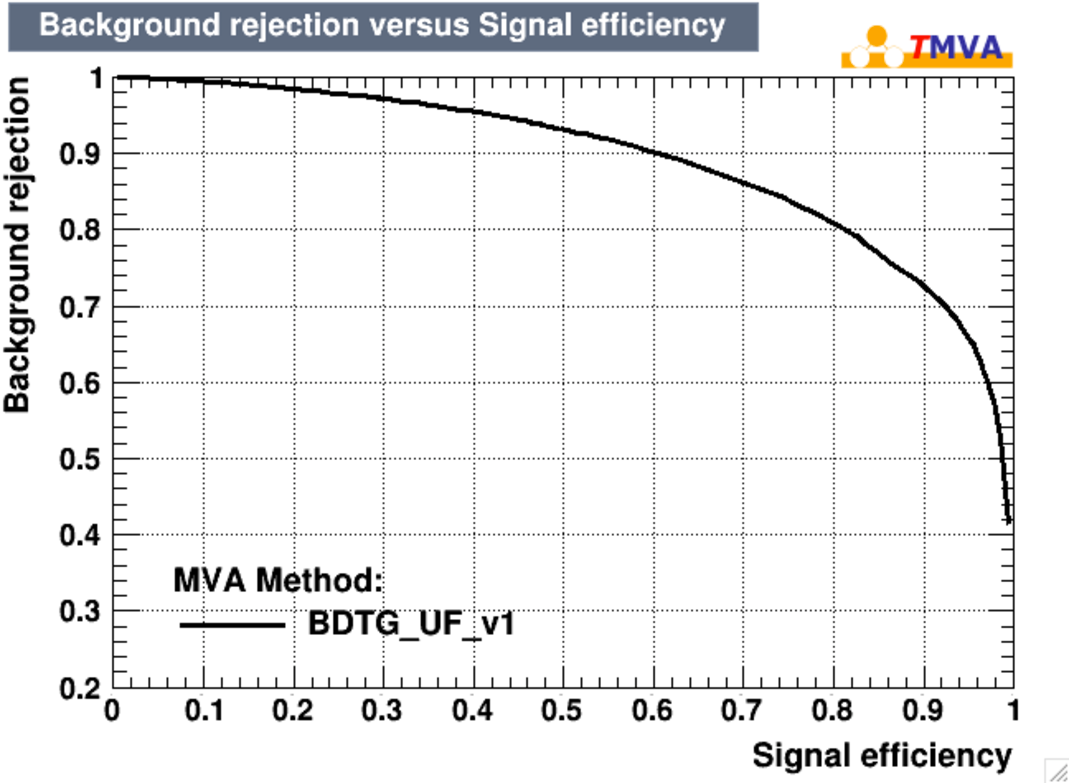
\includegraphics[width=0.5\linewidth]{figures/bdt_training/BDT_ROC_ge3j_all.pdf}
  \caption{The background-rejection vs. signal efficiency ROC curve from the
           BDT output score for events with $\ge 0$ jets (top left), $\le 1$ jet (top right),
           $= 2$ jets (bottom left), and $\ge 3$ jets (bottom right).}
  \label{fig:BDT_ROC}
\end{figure}

\clearpage

\section{Event categorization using Boosted Decision Trees}
\label{bdt_cats}

In order to optimize the sensitivity of the \Htomm search in a systematic way, the events
are categorized based on two criteria: the BDT output score and the muon eta information.
The output score of the BDT is used to separate signal
from background events, where the score ranges from -1 (background-like) to +1 (signal-like).
In addition, the maximum $|\eta|$ value of the two candidate muons is used to isolate events with better
signal-peak resolution. In order to optimize the choice of BDT and $|\eta|$ cuts, we designed and implemented
a decision tree autocategorizer to create categories by greedily optimizing a metric corresponding
to the sensitivity which by proxy minimizes the expected upper limit. The BDT training and the autocategorization
are performed on 50\% of the signal MC events and 100\% of the background MC events.
After training the autocategorizer on the signal and background MC to determine the categories,
the expected limits are calculated using data and the remaining 50\% of simulated signal events. Separating the
signal into separate training and evaluation sets and excluding the data from the training phase ensure an unbiased estimate for the expected limits.

\begin{figure}[hbp]
  \centering
  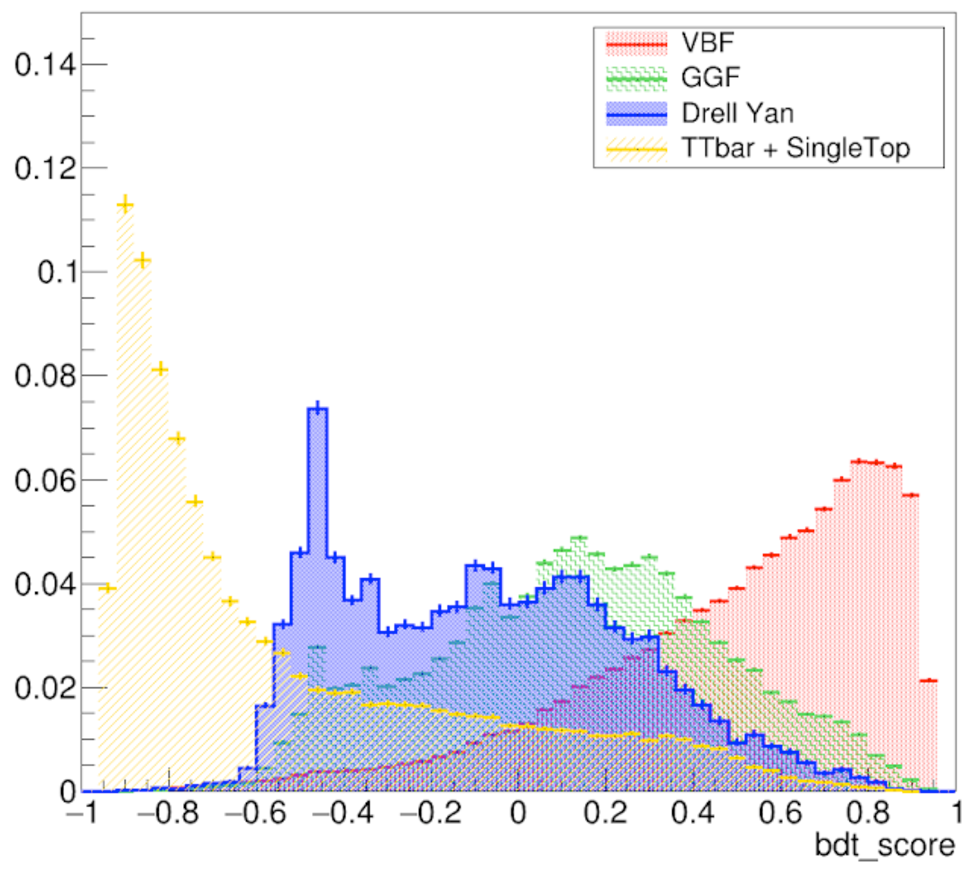
\includegraphics[width=0.49\linewidth]{figures/bdt_cats/bdt_score_ggH_VBF_DY_ttbar.pdf}
  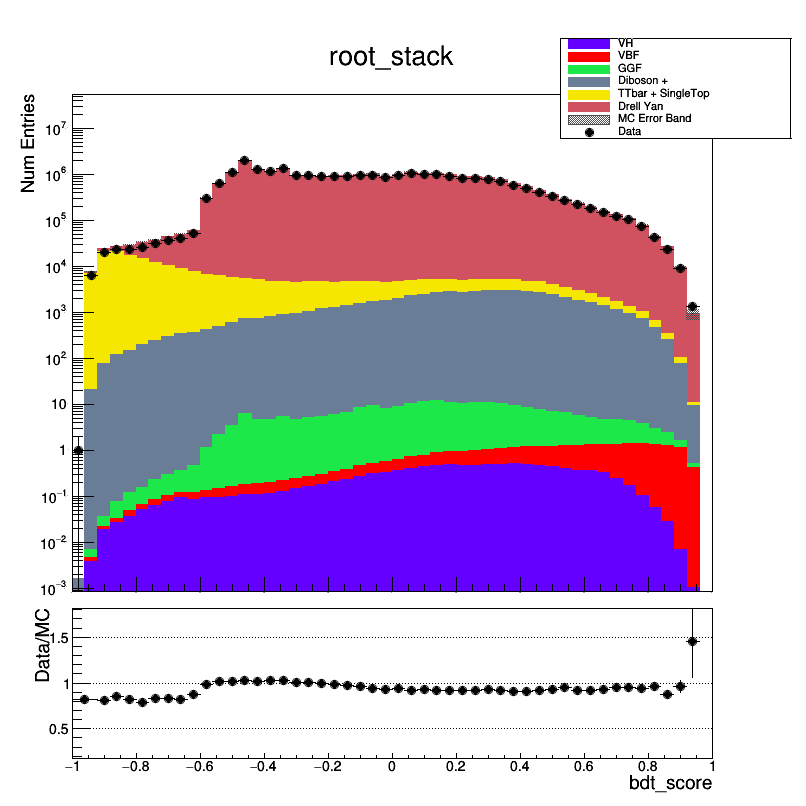
\includegraphics[width=0.49\linewidth]{figures/bdt_cats/bdt_score_inclusive_data_mc.png}
  \caption
   {The BDT score on the signal and background Monte Carlo (left), where a higher score marks the signal like events.
    Note \ttbar on the left as the most distinguishable background and VBF on the right as the most distinguishable signal.
    The BDT score in data is modeled well by the amc@NLO Drell--Yan MC (right). }
  \label{fig:bdt_score_inclusive}
\end{figure}

\subsection{The Auto-Categorizer}

In order to account for the resolution, the signal and background events are binned in half-GeV bins in the signal
region of the dimuon mass spectrum, 120 to 130 GeV. The significance in each bin is then given by $S/\sqrt{B}$.
The significance for independent bins adds in quadrature, so the net significance is given by

\begin{equation}
Net~Significance = \sum_{c,i}S_{c,i}^{2}/B_{c,i}
\end{equation}

where $i$ labels the bin in the signal region, and $c$ denotes the category. $S_{c,i}$ is the number of expected signal
events in the $i^{th}$ bin in that category, and $B_{i,c}$ is the number of expected background events in the $i^{th}$ bin.
By binning finely enough, the central mass bins contribute the most and the resolution is accounted for.

\begin{figure}[hbp]
  \centering
  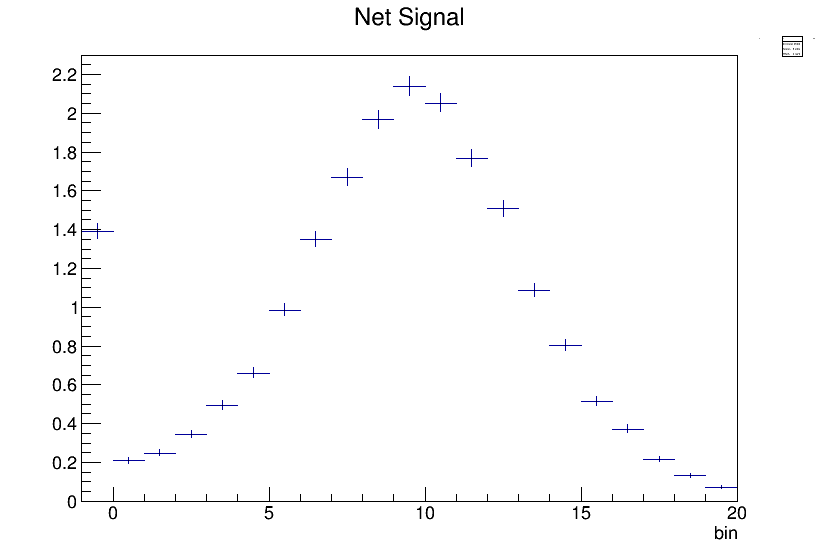
\includegraphics[width=0.49\linewidth]{figures/bdt_cats/binning_signal_example.png}
  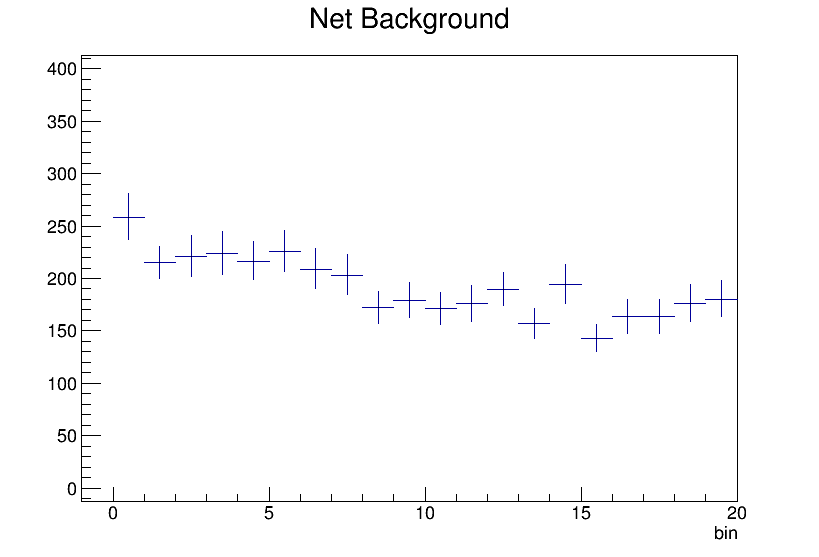
\includegraphics[width=0.49\linewidth]{figures/bdt_cats/binning_bg_example.png}
  \caption
  {An example of the binned signal and background necessary for the significance metric. The binning keeps the most sensitive bins
   from being drowned out by the others, providing a measure that accounts for both signal--background discrimination and resolution.}
  \label{fig:binning_example}
\end{figure}

On the first iteration, the autocategorizer calculates the net significance for the set of all events, the inclusive set.
The algorithm then searches over the inclusive set, checking all possible split values of the maximum muon $|\eta|$. Events
with maximum $|\eta|$ values less than the split go in one candidate category, and those with eta values greater than or equal
to the split value go into the other candidate category. For every split candidate, the algorithm calculates the net significance
in the two categories delineated by the split value. The maximum $|\eta|$ cut value that provides the largest gain in significance
over the inclusive set is stored. The gain is defined in the equation below where $c1$ and $c2$ are the prospective categories
created from $c$ by splitting on the feature.

\begin{equation}
Gain = \sum_{i}S_{c1,i}^{2}/B_{c1,i} + \sum_{i}S_{c2,i}^{2}/B_{c1,i} - \sum_{i}S_{c,i}^{2}/B_{c,i}
\end{equation}

The autocategorizer then searches over the BDT score values and stores the BDT score that provides the largest gain in significance.
The algorithm chooses to split on either the maximum muon $|\eta|$ or the BDT score (whichever has the higher gain), creating two
categories from the inclusive set of events. At the next iteration, the autocategorizer repeats the procedure for the two new
categories and chooses to split the category that provides the most gain. This process continues, each time greedily choosing to
split the category with the most gain, until the number of categories desired is reached.

%% \begin{figure}[hbp]
%%   \centering
%%   \includegraphics[width=0.49\linewidth]{figures/bdt_cats/split_example.png}
%%   \caption
%%    {Splitting a category on a feature to form two new categories.}
%%   \label{fig:split_example}
%% \end{figure}

\subsection{Final Categories}

After training the BDT and autocategorizing based upon the maximum muon $\eta|$ and the BDT score, the resulting categorization is
simplified by merging a few categories and rounding some of the cuts. Care is taken so that the simplifications do not worsen the
expected limit. The 13 finalized BDT categories in Figure~\ref{fig:final_categories} show a 23\% improvement compared to using the
15 Run~I \Htomm categories. The expected upper limits are evaluated on the same 36~\invfb of 2016 data and signal Monte Carlo in the
same way for an even comparison. The BDT categories are named such that the numbers go from low sensitivity to high sensitivity, e.g.
c0 has the lowest expected sensitivity and c12 has the highest expected sensitivity.

\begin{figure}[hbp]
  \centering
  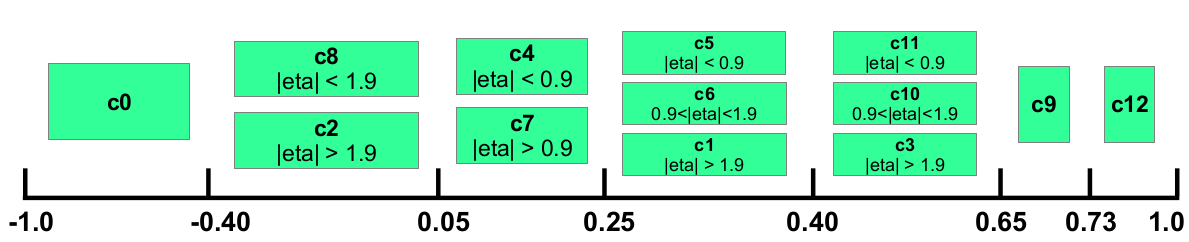
\includegraphics[width=1.0\linewidth]{figures/bdt_cats/final_categories.png}
  \caption
   {The final categorization. $|\eta|$ refers to the maximum $|\eta|$ value of the two muons in the dimuon pair. c12 and c9
    contain the highest proportion of VBF signal events.}
  \label{fig:final_categories}
\end{figure}

%\begin{table}[htb]
%  \caption{Expected signal and background yields near the signal peak, expected sensitivity from MC, and expected limits from data.}
%  \label{tab:cat_yields}
%  \begin{center}
%    \begin{tabular}{|c|r|r|c|c|c|r|}
%      \hline\hline
%      Category  & Signal  & Background & $\mathrm{S / B}$ (\%) & $\mathrm{S / \sqrt{B}}$ & Sensitivity & Limit \\  %% & Signal events
%      \hline\hline
%      c0        &  13.47  & 13660.7    & 0.098                 & 0.115                   & 0.124       & 19.30 \\  %% &  19.21
%      c1        &   3.74  &   982.5    & 0.381                 & 0.119                   & 0.130       & 19.80 \\  %% &   5.48
%      c2        &  14.97  &  7961.8    & 0.188                 & 0.167                   & 0.179       & 15.30 \\  %% &  21.97
%      c3        &   4.15  &   807.8    & 0.513                 & 0.146                   & 0.173       & 14.80 \\  %% &   5.95
%      c4        &   9.89  &  1516.0    & 0.652                 & 0.254                   & 0.271       &  8.47 \\  %% &  13.79
%      c5        &   9.46  &  1145.7    & 0.826                 & 0.279                   & 0.302       &  7.66 \\  %% &  12.56
%      c6        &  14.19  &  2270.6    & 0.625                 & 0.297                   & 0.323       &  7.28 \\  %% &  20.44
%      c7        &  27.40  &  6907.3    & 0.396                 & 0.329                   & 0.356       &  6.72 \\  %% &  40.39
%      c8        &  37.88  & 11766.1    & 0.322                 & 0.349                   & 0.374       &  6.25 \\  %% &  52.26
%      c9        &   6.22  &   400.2    & 1.555                 & 0.311                   & 0.345       &  7.59 \\  %% &   8.97
%      c10       &  14.05  &  1575.3    & 0.891                 & 0.354                   & 0.380       &  6.53 \\  %% &  20.75
%      c11       &  10.25  &   812.2    & 1.262                 & 0.359                   & 0.388       &  6.34 \\  %% &  13.91
%      c12       &   9.67  &   407.6    & 2.373                 & 0.479                   & 0.550       &  4.67 \\  %% &  14.33
%      %% \hline
%      %% Inclusive & 170.16  & 45540.3    & 0.373                 & 0.797                   & 0.858       &  1.85 \\  %% & 250.07
%      \hline\hline
%    \end{tabular}
%  \end{center}
%\end{table}

\begin{table}[htb]
  \caption{Full Width Half Max (FWHM) of the signal peak, expected signal and background yields within the FWHM,
           expected sensitivity from MC, and expected limits from data}
  \label{tab:cat_yields}
  \begin{center}
    \begin{tabular}{|c|r|r|c|c|c|r|r|}
      \hline\hline
      Category  & Signal FWHM (GeV) & Signal & Background & $\mathrm{S / B}$ (\%) & $\mathrm{S / \sqrt{B}}$ & Sensitivity & Limit \\  %% & Signal events
      \hline\hline
      c0          &        4.4           &      13.4826         &    14187.6        &     0.000950307    &     0.113193        & 0.124       & 19.30 \\
      c1          &        5.8           &      3.52888         &    970.875        &     0.00363474     &     0.113255        & 0.130       & 19.80 \\
      c2          &        5.8           &      14.2112         &    8248.64        &     0.00172286     &     0.156473        & 0.179       & 15.30 \\
      c3          &        6.0           &      3.82012         &    779.594        &     0.00490015     &     0.136818        & 0.173       & 14.80 \\
      c4          &        3.0           &      9.92363         &    1609.08        &     0.00616729     &     0.24739         & 0.271       &  8.47 \\
      c5          &        2.8           &      8.5825          &    1028.08        &     0.00834811     &     0.267671        & 0.302       &  7.66 \\
      c6          &        4.0           &      14.1224         &    2371.09        &     0.00595611     &     0.290025        & 0.323       &  7.28 \\
      c7          &        4.2           &      26.3575         &    6904.16        &     0.00381762     &     0.317211        & 0.356       &  6.72 \\
      c8          &        3.6           &      35.6493         &    11187.4        &     0.00318655     &     0.337043        & 0.374       &  6.25 \\
      c9          &        4.0           &      6.12457         &    451.281        &     0.0135715      &     0.288305        & 0.345       &  7.59 \\
      c10         &        4.0           &      13.9349         &    1667.59        &     0.00835632     &     0.34124         & 0.380       &  6.53 \\
      c11         &        3.0           &      9.59255         &    765.226        &     0.0125356      &     0.346768        & 0.388       &  6.34 \\
      c12         &        4.0           &      9.58541         &    420.983        &     0.0227691      &     0.467173        & 0.550       &  4.67 \\
      \hline\hline
    \end{tabular}
  \end{center}
\end{table}


\subsection{Validating The Categories}

It is important that the signal is correctly modeled in each category in order to report an accurate expected upper limit.
%% Insofar, the Monte Carlo is compared to the Data in the sidebands.
Figure~\ref{fig:valid_bdt_incl} shows the data-to-MC agreement for the BDT features
for the inclusive set of events with dimuon mass greater than 60~GeV.

\begin{figure}[hbp]
  \centering
  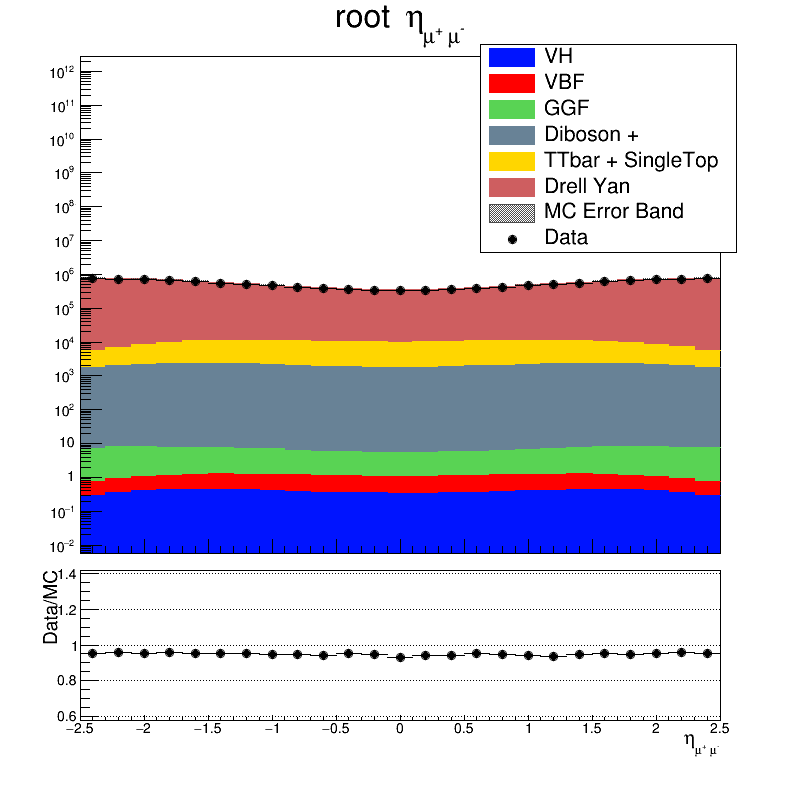
\includegraphics[width=0.32\linewidth]{figures/bdt_cats/dimu_eta_root.png}
  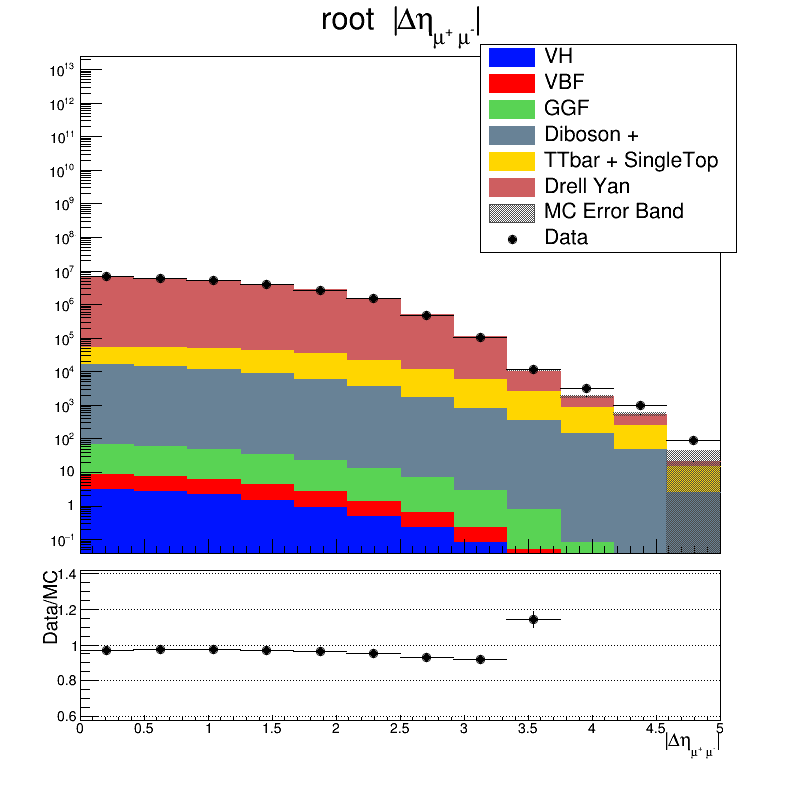
\includegraphics[width=0.32\linewidth]{figures/bdt_cats/dimu_abs_dEta_root.png}
  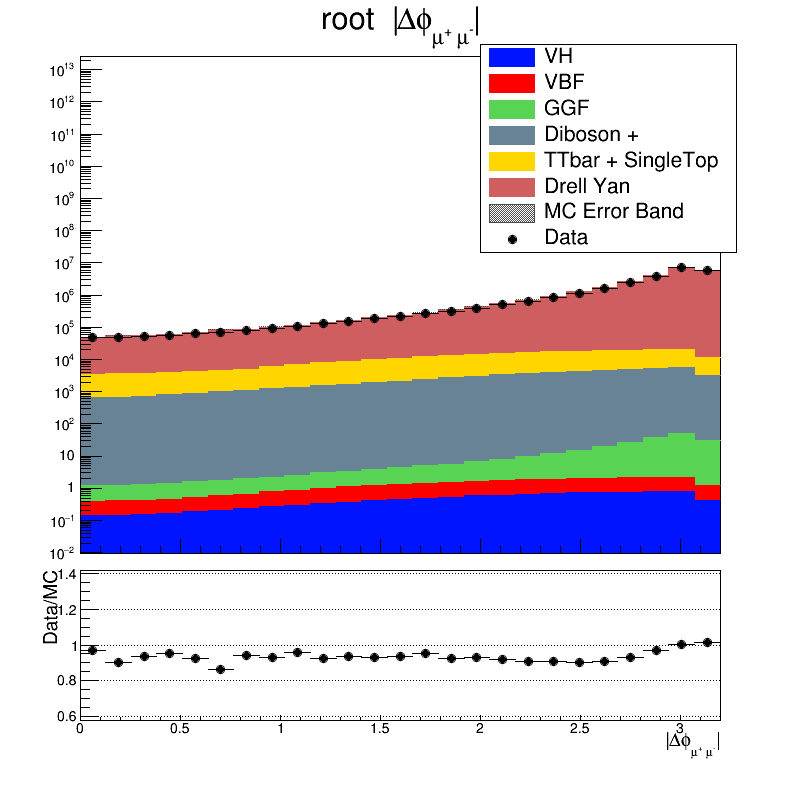
\includegraphics[width=0.32\linewidth]{figures/bdt_cats/dimu_abs_dPhi_root.png}
  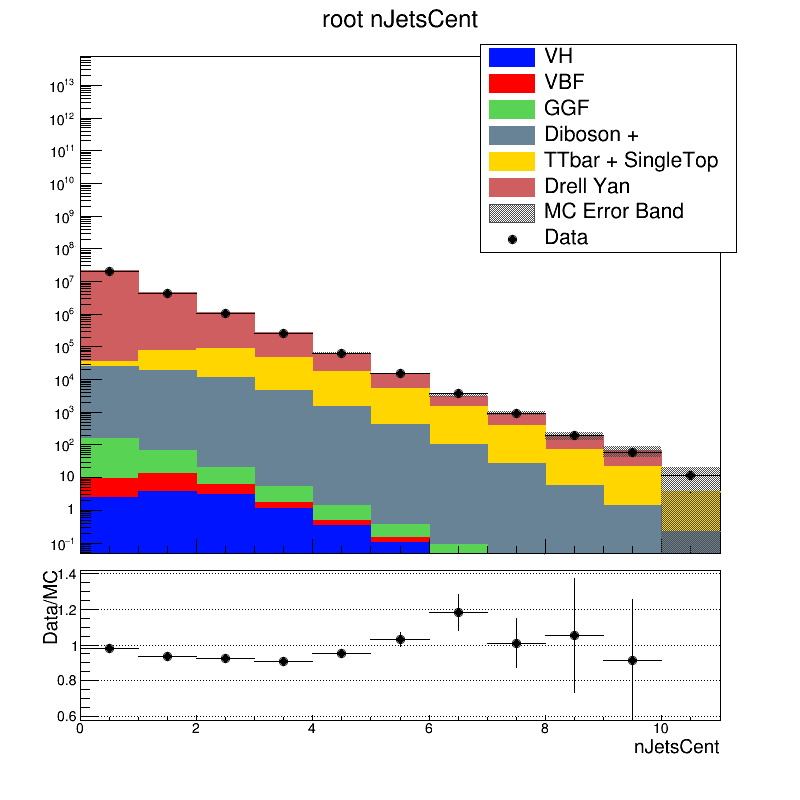
\includegraphics[width=0.32\linewidth]{figures/bdt_cats/nJetsCent_root.png}
  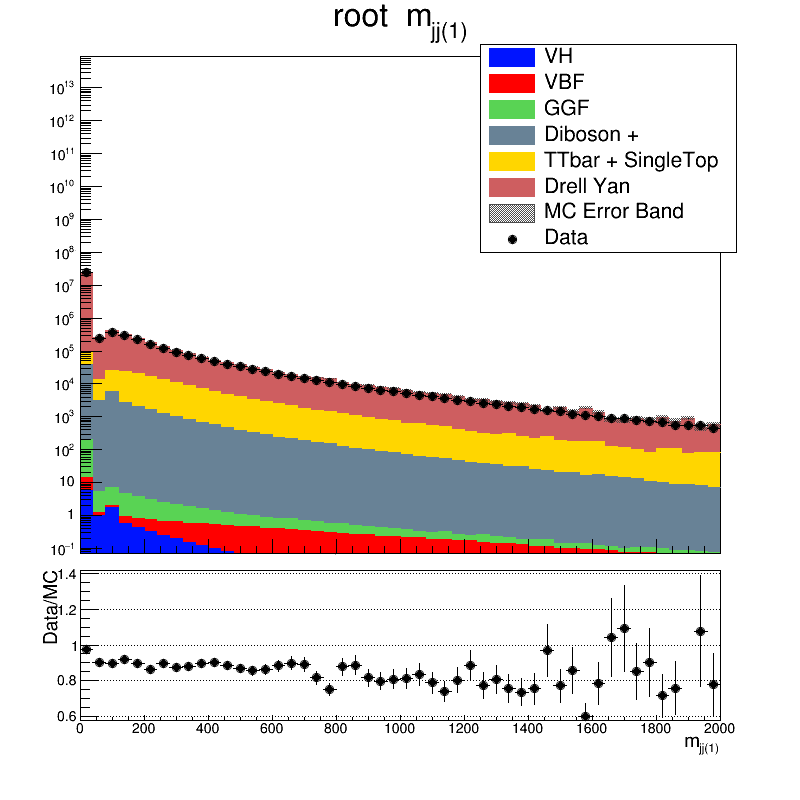
\includegraphics[width=0.32\linewidth]{figures/bdt_cats/dijet1_mass_root.png}
  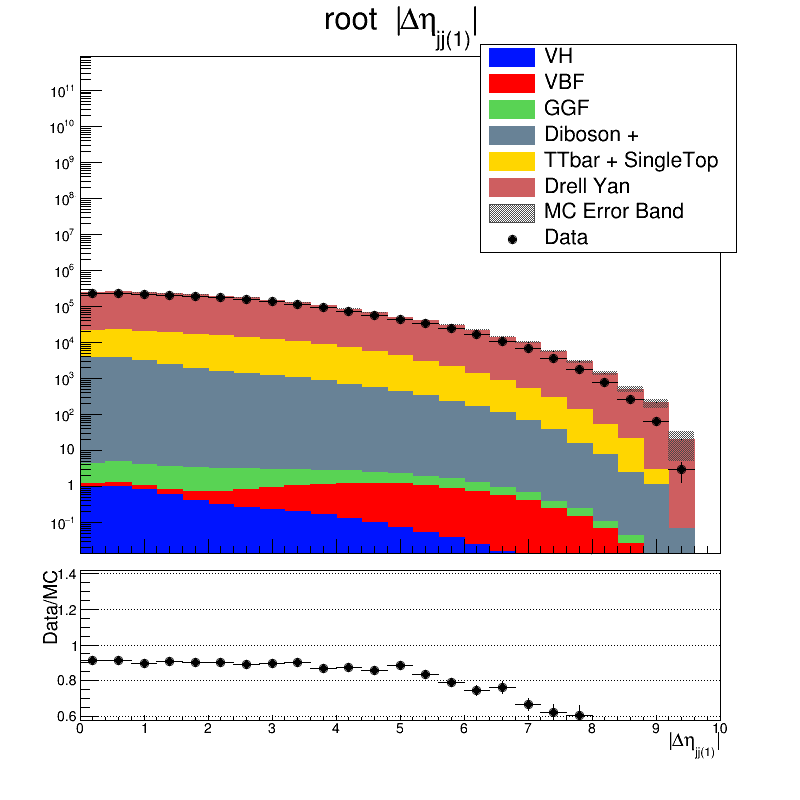
\includegraphics[width=0.32\linewidth]{figures/bdt_cats/dijet1_abs_dEta_root.png}
  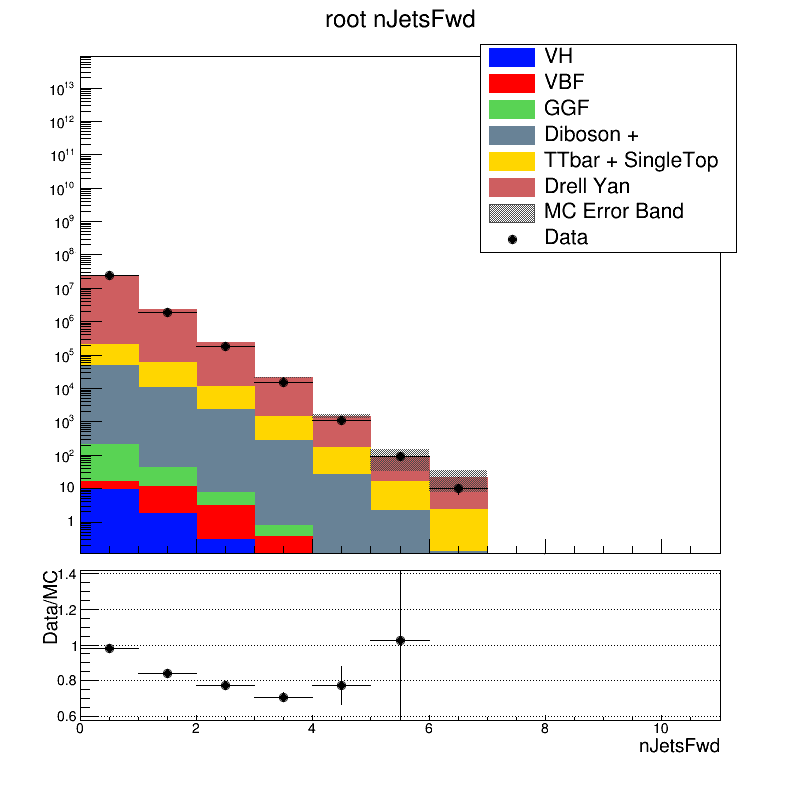
\includegraphics[width=0.32\linewidth]{figures/bdt_cats/nJetsFwd_root.png}
  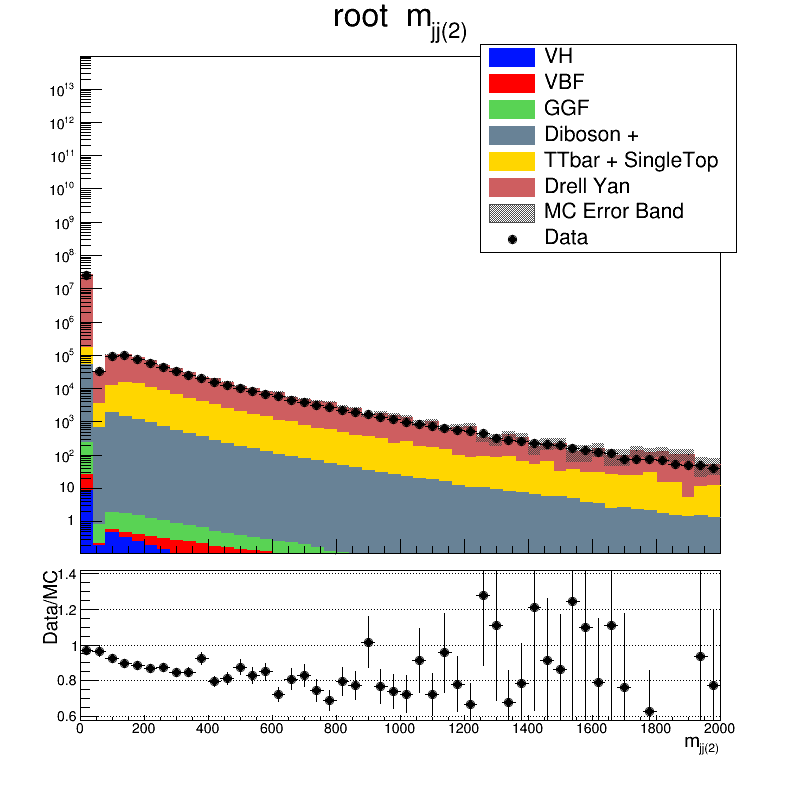
\includegraphics[width=0.32\linewidth]{figures/bdt_cats/dijet2_mass_root.png}
  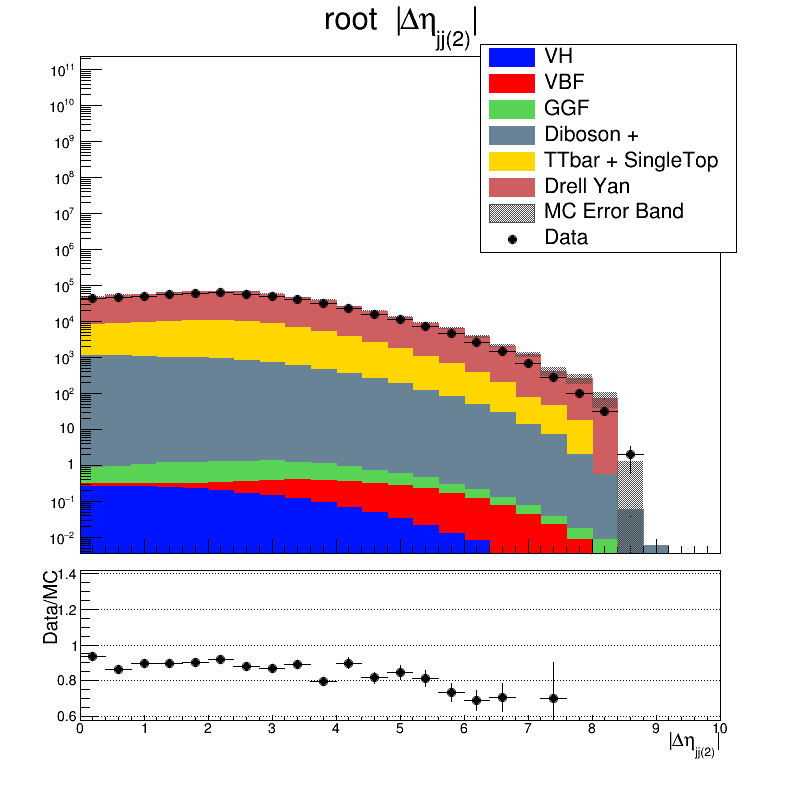
\includegraphics[width=0.32\linewidth]{figures/bdt_cats/dijet2_abs_dEta_root.png}
  \caption
   {Validation of BDT input variables in inclusive events.}
  \label{fig:valid_bdt_incl}
\end{figure}

The Data and Monte Carlo agree very well especially in the dimuon mass distribution, where the agreement is within 5\%.
Furthermore, Fig.~\ref{fig:valid_bdt_c12a} and~\ref{fig:valid_bdt_c12b} show the Data/MC agreement for c12,
the most sensitive, most VBF-like category. The BDT distribution in quantile is presented in Fig.~\ref{fig:bdt_quantile}
with the systematic uncertainties given by the JES and PU.

\begin{figure}[hbp]
  \centering
  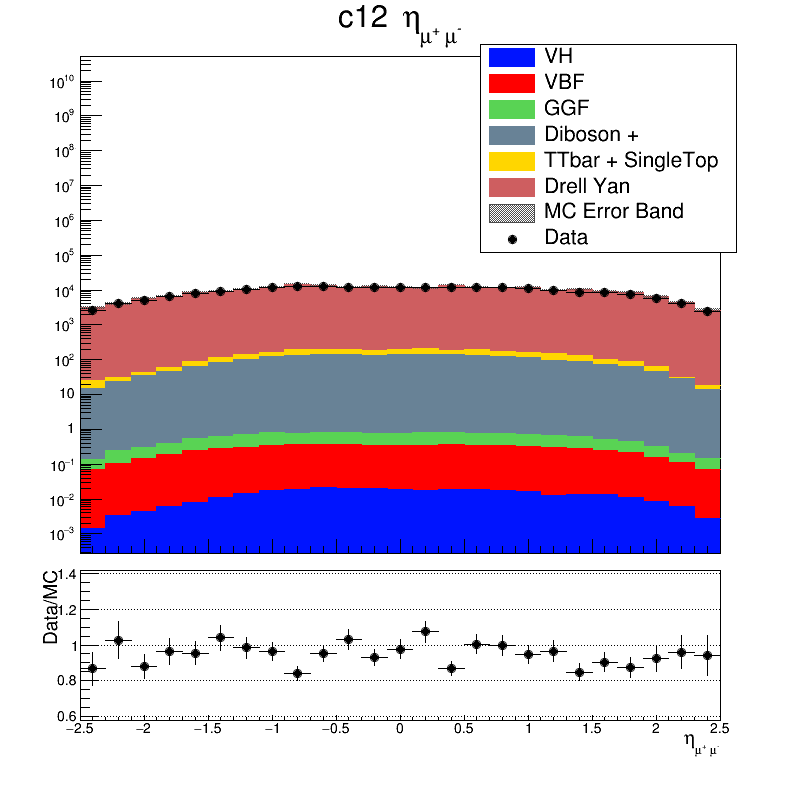
\includegraphics[width=0.32\linewidth]{figures/bdt_cats/dimu_eta_c12.png}
  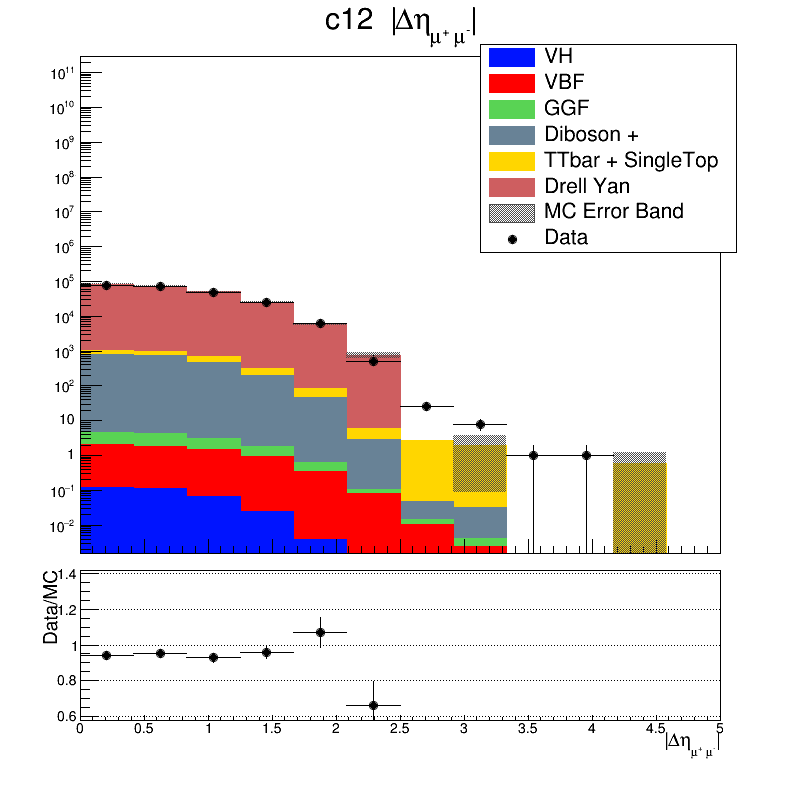
\includegraphics[width=0.32\linewidth]{figures/bdt_cats/dimu_abs_dEta_c12.png}
  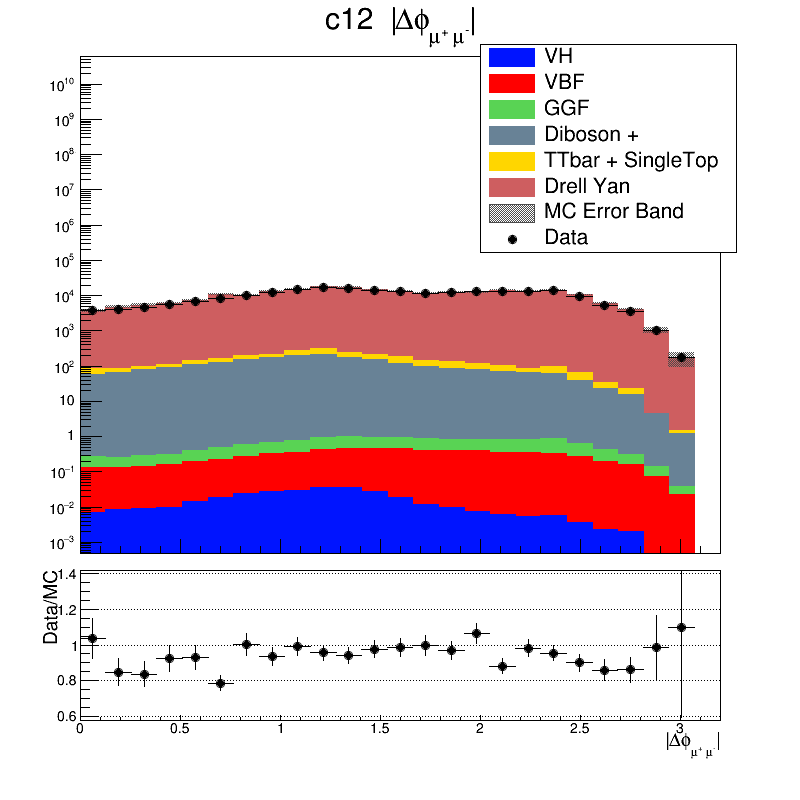
\includegraphics[width=0.32\linewidth]{figures/bdt_cats/dimu_abs_dPhi_c12.png}
  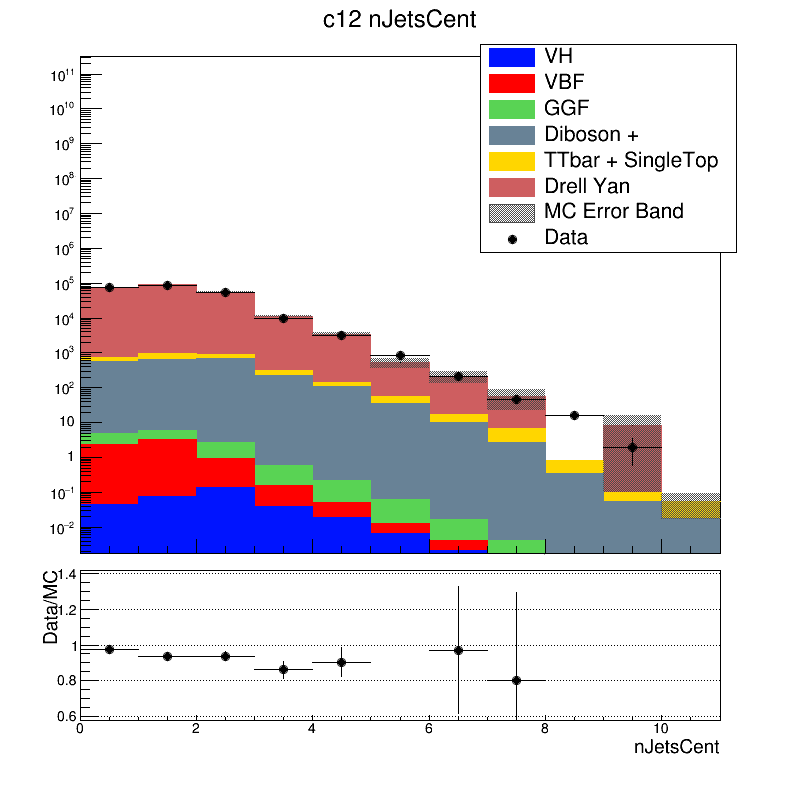
\includegraphics[width=0.32\linewidth]{figures/bdt_cats/nJetsCent_c12.png}
  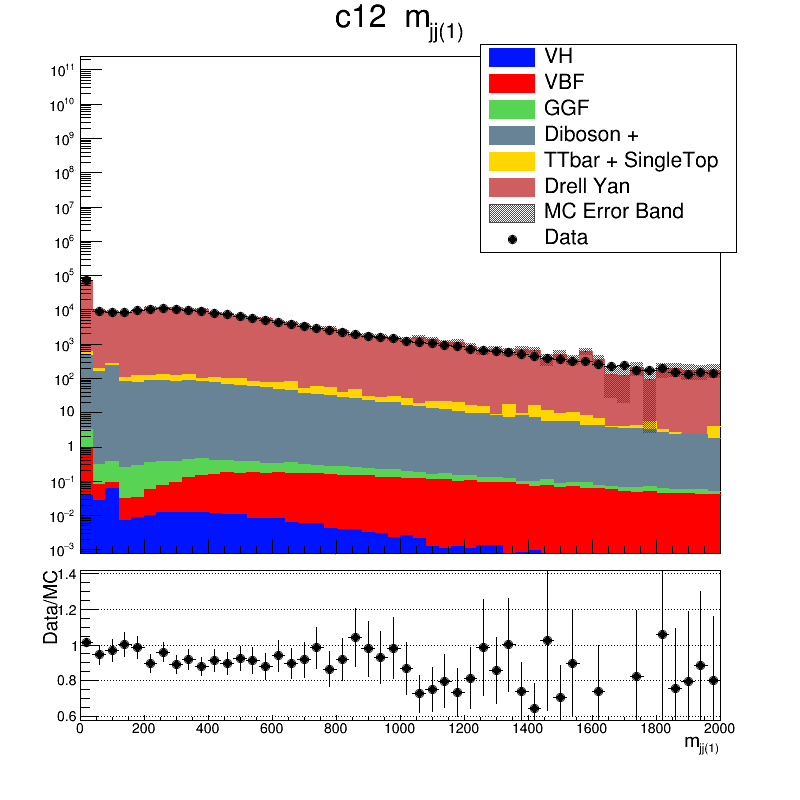
\includegraphics[width=0.32\linewidth]{figures/bdt_cats/dijet1_mass_c12.png}
  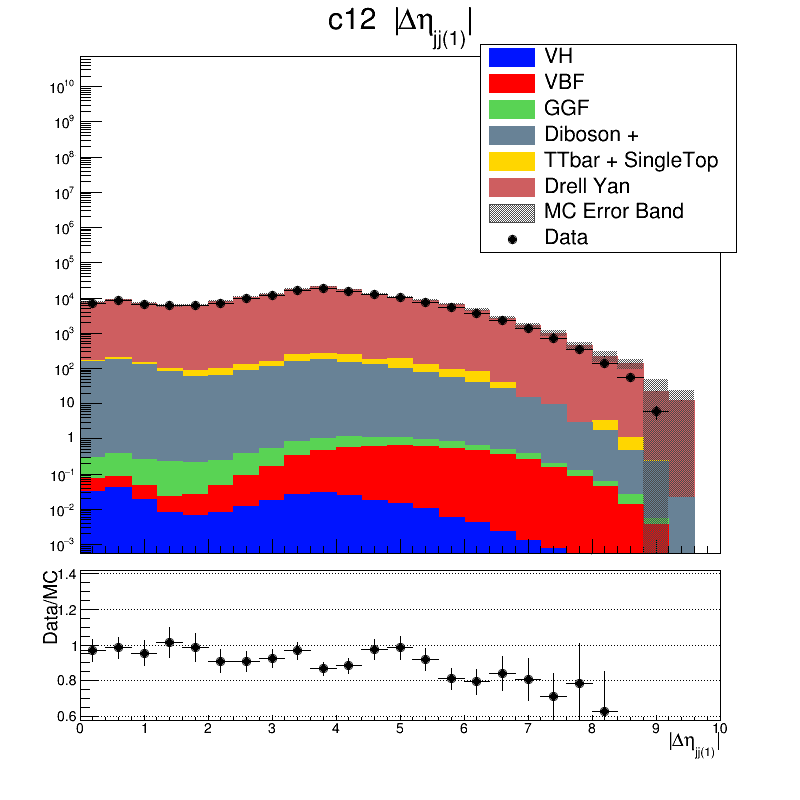
\includegraphics[width=0.32\linewidth]{figures/bdt_cats/dijet1_abs_dEta_c12.png}
  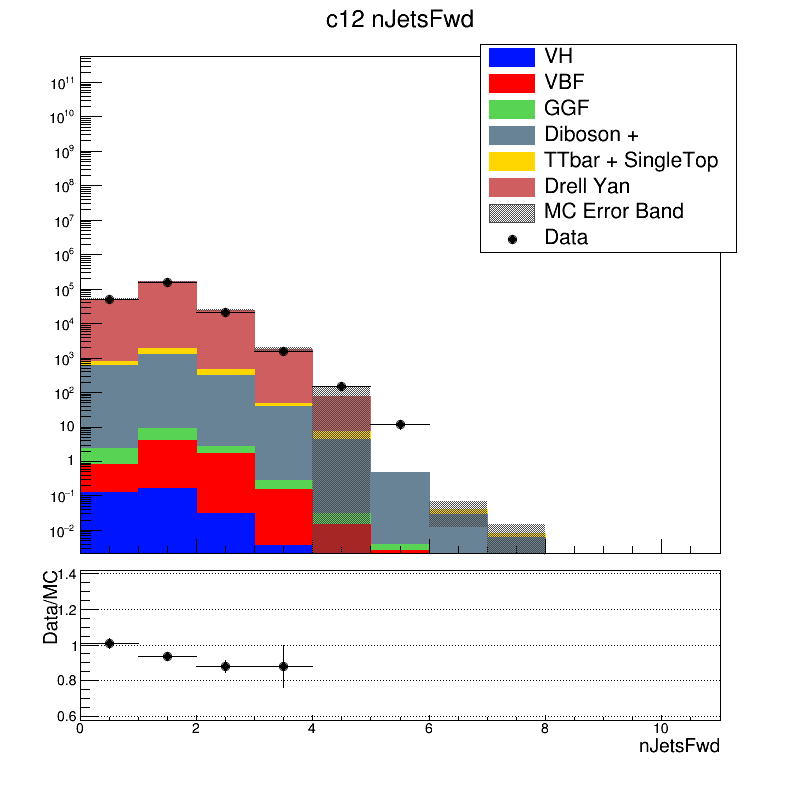
\includegraphics[width=0.32\linewidth]{figures/bdt_cats/nJetsFwd_c12.png}
  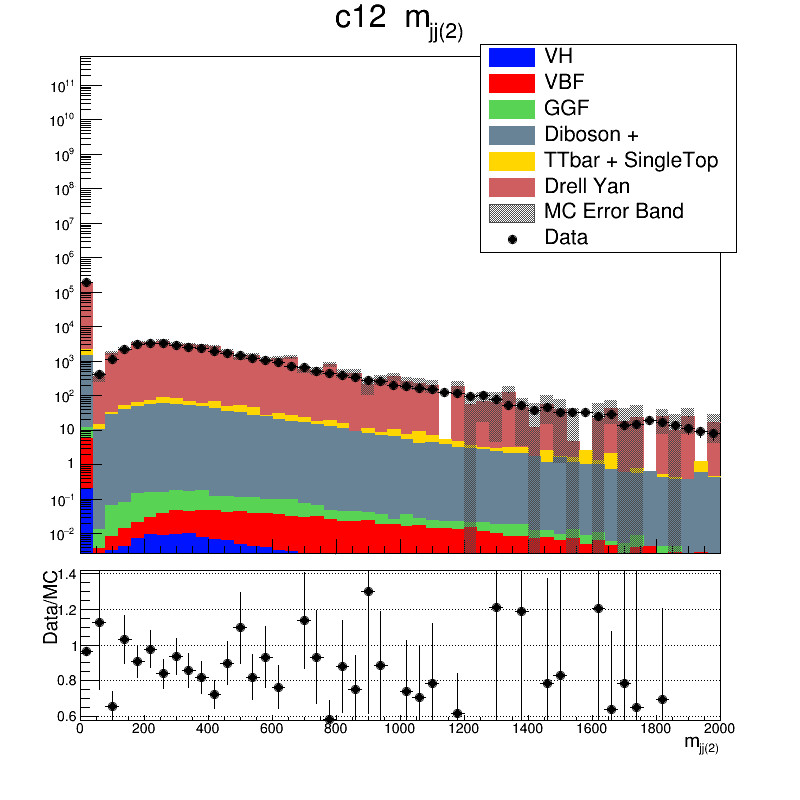
\includegraphics[width=0.32\linewidth]{figures/bdt_cats/dijet2_mass_c12.png}
  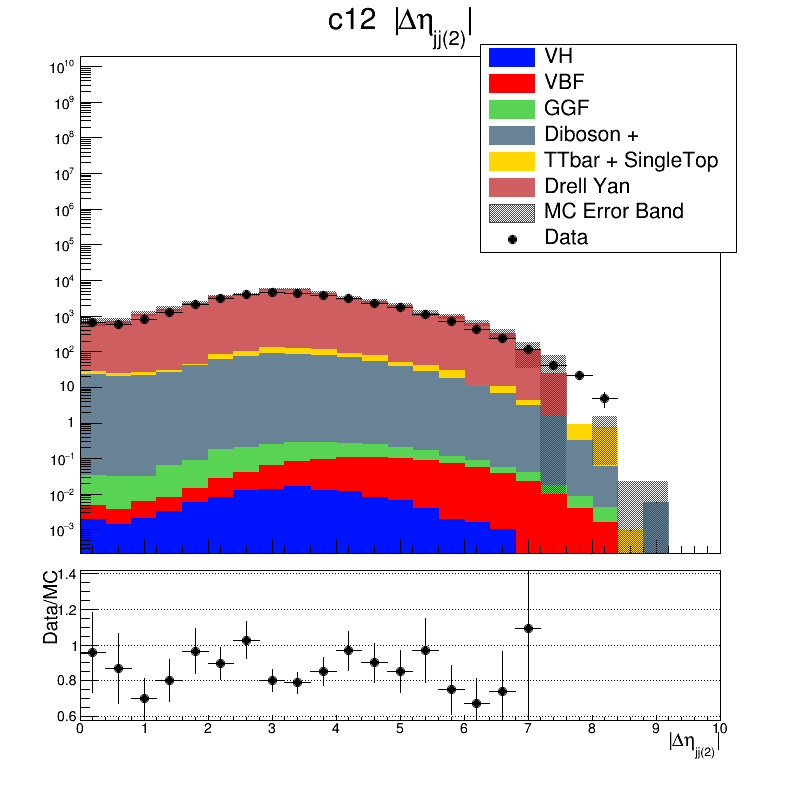
\includegraphics[width=0.32\linewidth]{figures/bdt_cats/dijet2_abs_dEta_c12.png}
  \caption
   {Data/MC agreement for the most sensitive category.}
  \label{fig:valid_bdt_c12a}
\end{figure}

\begin{figure}[hbp]
  \centering
  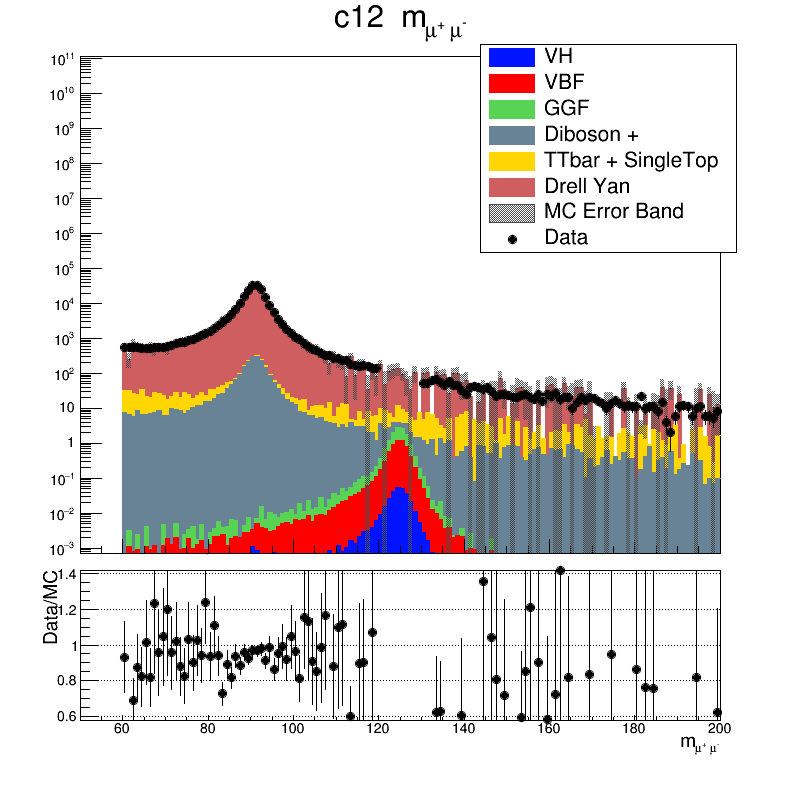
\includegraphics[width=0.32\linewidth]{figures/bdt_cats/dimu_mass_Roch_c12.png}
  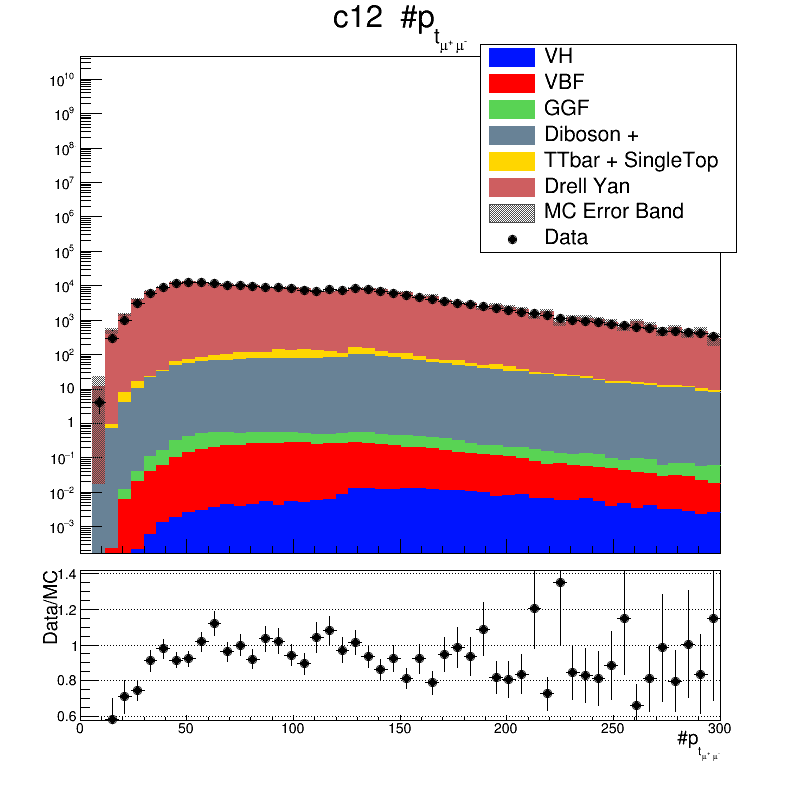
\includegraphics[width=0.32\linewidth]{figures/bdt_cats/dimu_pt_c12.png}
  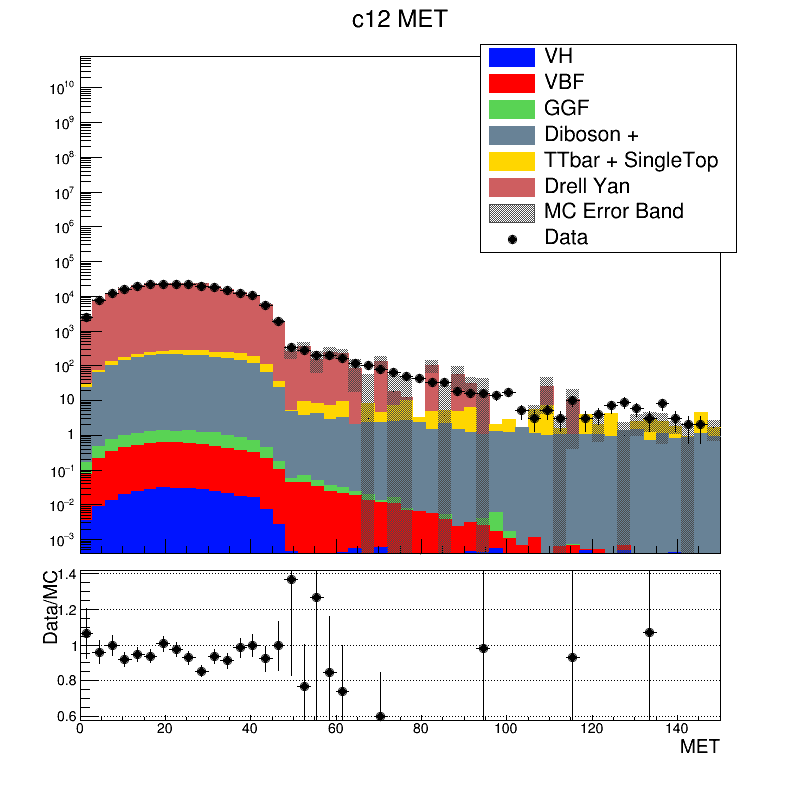
\includegraphics[width=0.32\linewidth]{figures/bdt_cats/MET_c12.png}
  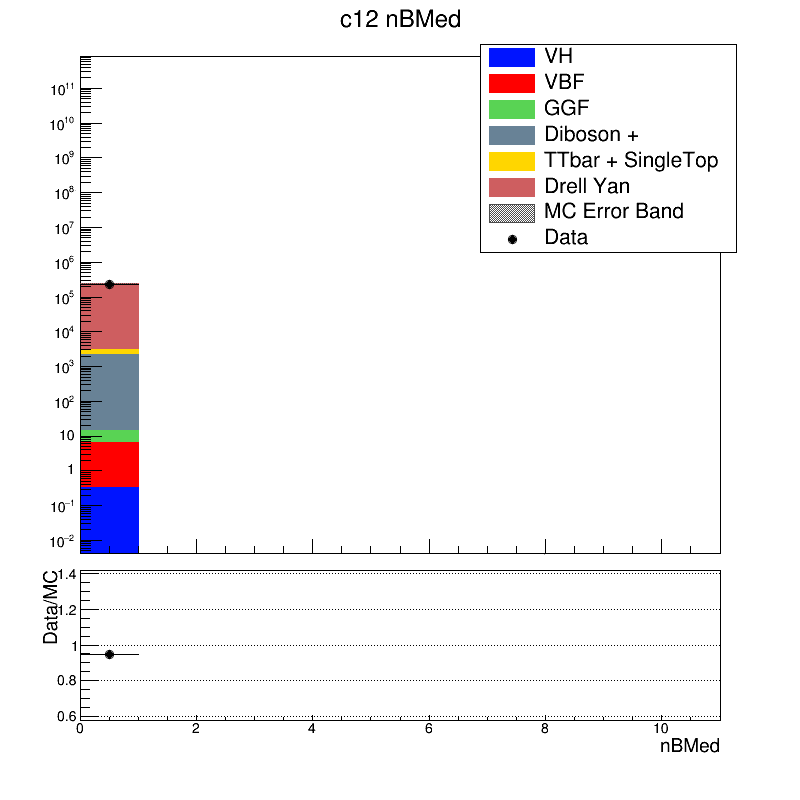
\includegraphics[width=0.32\linewidth]{figures/bdt_cats/nBMed_c12.png}
  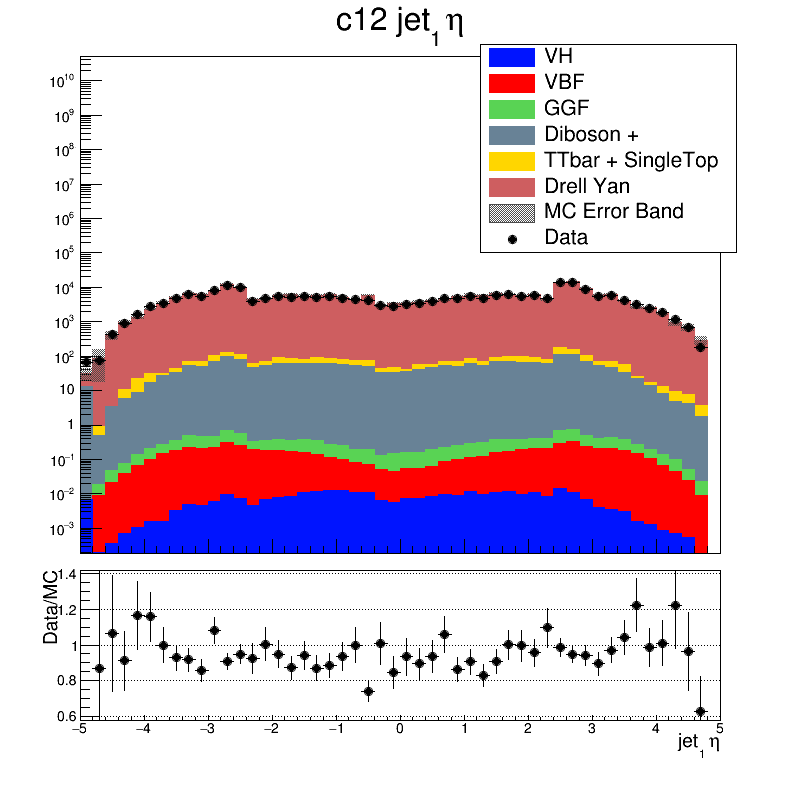
\includegraphics[width=0.32\linewidth]{figures/bdt_cats/jet1_eta_c12.png}
  \includegraphics[width=0.32\linewidth]{figures/bdt_cats/jet2_eta_c12.png}
  \caption
   {Data/MC agreement for the most sensitive category.}
  \label{fig:valid_bdt_c12b}
\end{figure}

\begin{figure}[hbp]
\centering
\includegraphics[width=0.7\linewidth]{figures/bdt_cats/BdtOnH_QM_bkg.png}
  \caption{The BDT distribution in quantile in data and MC. The systematic uncertainty is given by the JES and PU.}
  \label{fig:bdt_quantile}
\end{figure}

Again, the Data and Monte Carlo agree very well. Lastly, it is important that the BDT score is mass independent. One way to
show this is to demonstrate that the classifier score remains the same for signal Monte Carlo with different values of
$M_{Higgs}$. If the BDT score does not change as the mass changes, then it is clearly mass independent. As shown in
Figure~\ref{fig:mass_independence}, the BDT score does not change significantly with the dimuon mass.

\begin{figure}[hbp]
  \centering
  \includegraphics[width=0.49\linewidth]{figures/bdt_cats/BDT_Score_GGF_M125_vs_M120.png}
  \includegraphics[width=0.49\linewidth]{figures/bdt_cats/BDT_Score_GGF_M125_vs_M130.png}
  \includegraphics[width=0.49\linewidth]{figures/bdt_cats/BDT_Score_VBF_M125_vs_M120.png}
  \includegraphics[width=0.49\linewidth]{figures/bdt_cats/BDT_Score_VBF_M125_vs_M130.png}
  \caption
   {Plots showing the agreement between $M_{Higgs}$ = 125 GeV vs. 120 GeV and $M_{Higgs}$ = 125 GeV vs. 130 GeV for ggH and VBF.}
  \label{fig:mass_independence}
\end{figure}
